\documentclass[a4paper,12pt]{report}
\usepackage{graphicx}  % for including images
\usepackage{listings}  % for displaying code
\usepackage{caption}   % for captions of images
\usepackage{amsmath}   % for math equations
\usepackage{fancyhdr}  % for header and footer customization
\usepackage[hidelinks]{hyperref}
\usepackage[hyphens]{url} % for URLs
\usepackage{titlesec}
\usepackage[a4paper, margin=1in]{geometry}
\usepackage{float}
\usepackage{minted}

\setlength{\parindent}{0pt}
\lstset{
    basicstyle=\ttfamily\footnotesize,
    columns=fullflexible,
    keepspaces=true,
    breaklines=true,
    breakatwhitespace=true,
    postbreak=\mbox{\textcolor{red}{$\hookrightarrow$}\space},
}
% Configure hyperref to remove link colors
\hypersetup{
    colorlinks=false,   % Disables colored links
    pdfborder={0 0 0},  % Removes link borders
    linkcolor=black,    % Sets link color to black
    filecolor=black,    % Sets file link color to black
    urlcolor=black      % Sets URL color to black
}

\titleformat{\chapter}[hang]{\normalfont\huge\bfseries}{\thechapter}{2pc}{}
\titlespacing*{\chapter}{0pt}{-60pt}{20pt}

\title{Testing and Quality Analysis of\\commons-imaging Project\\ \\
\vspace{0.5cm}\href{https://github.com/nimamehranfar/commons-imaging}{\texttt{GitHub Repository}}\\}
\author{Nima Mehranfar}
\date{\today}

\begin{document}

% Title page
\maketitle

% Abstract
\begin{abstract}
    This report presents the testing and quality analysis conducted on the commons-imaging project hosted on GitHub. The project undergoes thorough software quality analysis, CI/CD pipeline setup, code coverage analysis, performance testing, mutation testing, security assessment, and more. The results of these analyses are presented along with the actions taken to improve the quality of the commons-imaging codebase.
\end{abstract}

% Table of contents
\tableofcontents
\newpage

% List of Figures
\listoffigures
\newpage

% List of Tables
\listoftables
\newpage

% Introduction
\chapter{Introduction}
The \textit{commons-imaging} project is a Java library developed by the Apache Software Foundation. It provides a comprehensive API for working with various image formats, enabling developers to read, write, and manipulate images with ease. This project focuses on evaluating the \textit{commons-imaging} codebase through a rigorous quality assurance process to ensure reliability, maintainability, and performance.

\section{Objectives}
This testing project aims to achieve the following objectives:
\begin{itemize}
    \item Establish CI/CD pipelines for the \textit{commons-imaging} project using GitHub Actions.
    \item Perform software quality analysis leveraging SonarCloud for static code evaluation and reporting.
    \item Develop a Docker image to facilitate streamlined deployment and testing environments.
    \item Conduct code coverage analysis using JaCoCo to identify untested areas in the codebase.
    \item Apply mutation testing with PiTest to evaluate the robustness of existing test cases.
    \item Execute stress testing on project components with JMH to assess performance under load.
    \item Generate automated test cases for inadequately tested code segments using Randoop.
    \item Perform security analysis using Snyk to detect and mitigate potential vulnerabilities.
\end{itemize}

\newpage

% CI/CD Pipeline Setup
\chapter{CI/CD Pipeline}
The \textit{commons-imaging} project has been integrated into a CI/CD pipeline that can be built both locally and on cloud servers, including GitHub. This pipeline automates the build, test, and deployment processes to ensure continuous integration and delivery, enabling efficient and reliable software updates.

\section{CI/CD Configuration}
The CI/CD pipeline configuration utilizes GitHub Actions to automate the workflow. Below is the YAML file for the GitHub Actions workflow configuration:

\begin{lstlisting}[language=java, caption=GitHub Actions Workflow Configuration (\texttt{maven.yml})]
name: Java CI

on: [push, pull_request, workflow_dispatch]

permissions:
  contents: read

jobs:
  build:
    runs-on: ${{ matrix.os }}
    continue-on-error: ${{ matrix.experimental }}
    strategy:
      matrix:
        os: [windows-latest, macos-13, ubuntu-latest]
        java: [8, 11, 17, 21]
        experimental: [false]
        include:
            - java: 23
              os: ubuntu-latest
              experimental: false
            - java: 24-ea
              os: ubuntu-latest
              experimental: true

    steps:
    # Configure Git settings to avoid line-ending issues
    - name: Prepare git
      run: |-
        git config --global core.autocrlf false
        git config --global core.eol lf
    - uses: actions/checkout@v2  # Checkout the repository code
      with:
        persist-credentials: false
    - name: Set up JDK ${{ matrix.java }}
      uses: actions/setup-java@v2  # Setup JDK version
      with:
        distribution: 'temurin'
        java-version: ${{ matrix.java }}
    - name: Build with Maven
      run: mvn --errors --show-version --batch-mode --no-transfer-progress
\end{lstlisting}

\newpage


% Software Quality Analysis with SonarCloud
\chapter{Software Quality Analysis with SonarCloud}
The software quality analysis of the \textit{commons-imaging} project is conducted using SonarCloud, a powerful tool that identifies potential code quality issues and provides recommendations for improvements. By integrating SonarCloud into the development workflow, developers can continuously monitor and address various code quality aspects to ensure a robust and maintainable codebase.

\section{Issues Categorization}
SonarCloud categorizes the issues it identifies into three main types:
\begin{itemize}
    \item \textbf{Maintainability}: These refer to unnecessary complexity or suboptimal code patterns that may not be bugs but could lead to maintenance challenges.
    \item \textbf{Reliability}: Errors in the code that could lead to functional failures or unexpected behavior.
    \item \textbf{Security}: Potential security risks within the code that could be exploited by malicious actors.
\end{itemize}

\section{Refactoring and Rationale}
Several refactoring actions were undertaken to address the issues identified by SonarCloud. For those issues that were skipped, a clear rationale was provided. 

As illustrated in the image below (Figure \ref{fig:sonar_issues}), a total of 2325 issues were found, including 18 critical "blocker" severity issues and 333 "high" severity issues. All the "blocker" issues were maintainability; And I prioritized addressing some of the these issues to improve the overall code quality.

\begin{figure}[H]
    \centering
    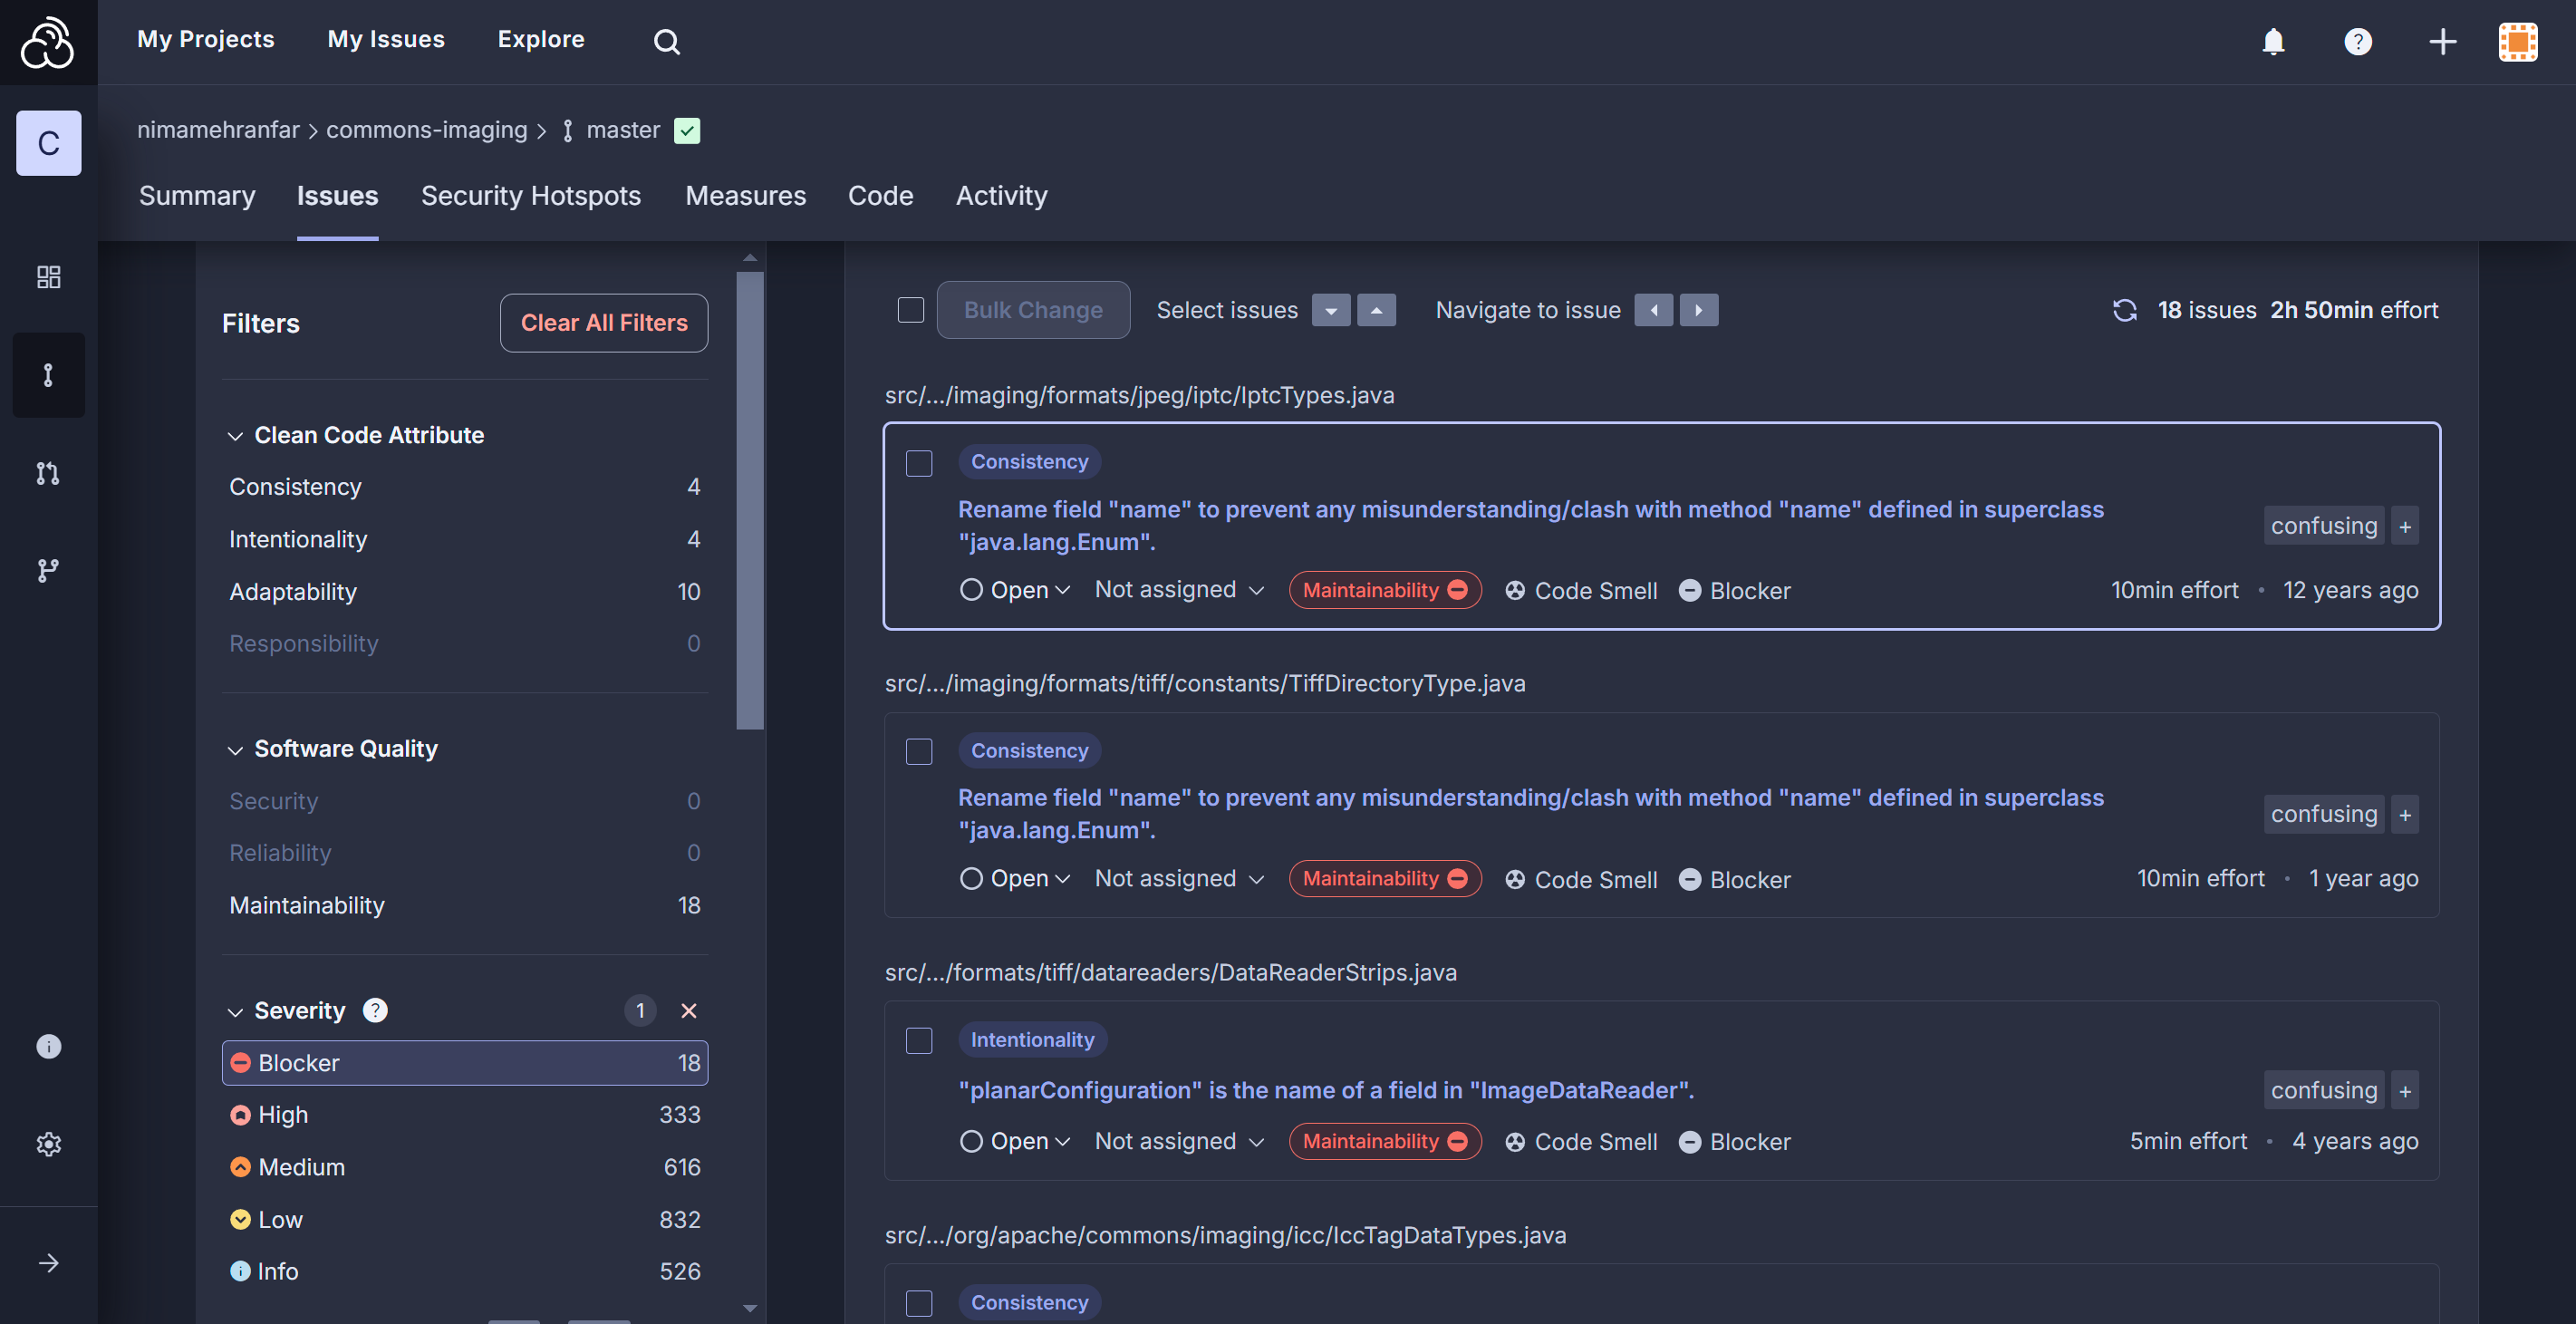
\includegraphics[width=1\textwidth]{Report_Img/SonarQube_issues.png}
    \caption{SonarCloud Issues Overview: 2325 issues detected, including blocker and high severity issues.}
    \label{fig:sonar_issues}
\end{figure}

Some of the common issues included a lack of assertions in test cases, confusing or duplicate method/variable names and missing break in switch cases, as demonstrated in the images below (Figures \ref{fig:assertion_issue}, \ref{fig:naming_issue}, \ref{fig:missing_break_issue}).

\begin{figure}[H]
    \centering
    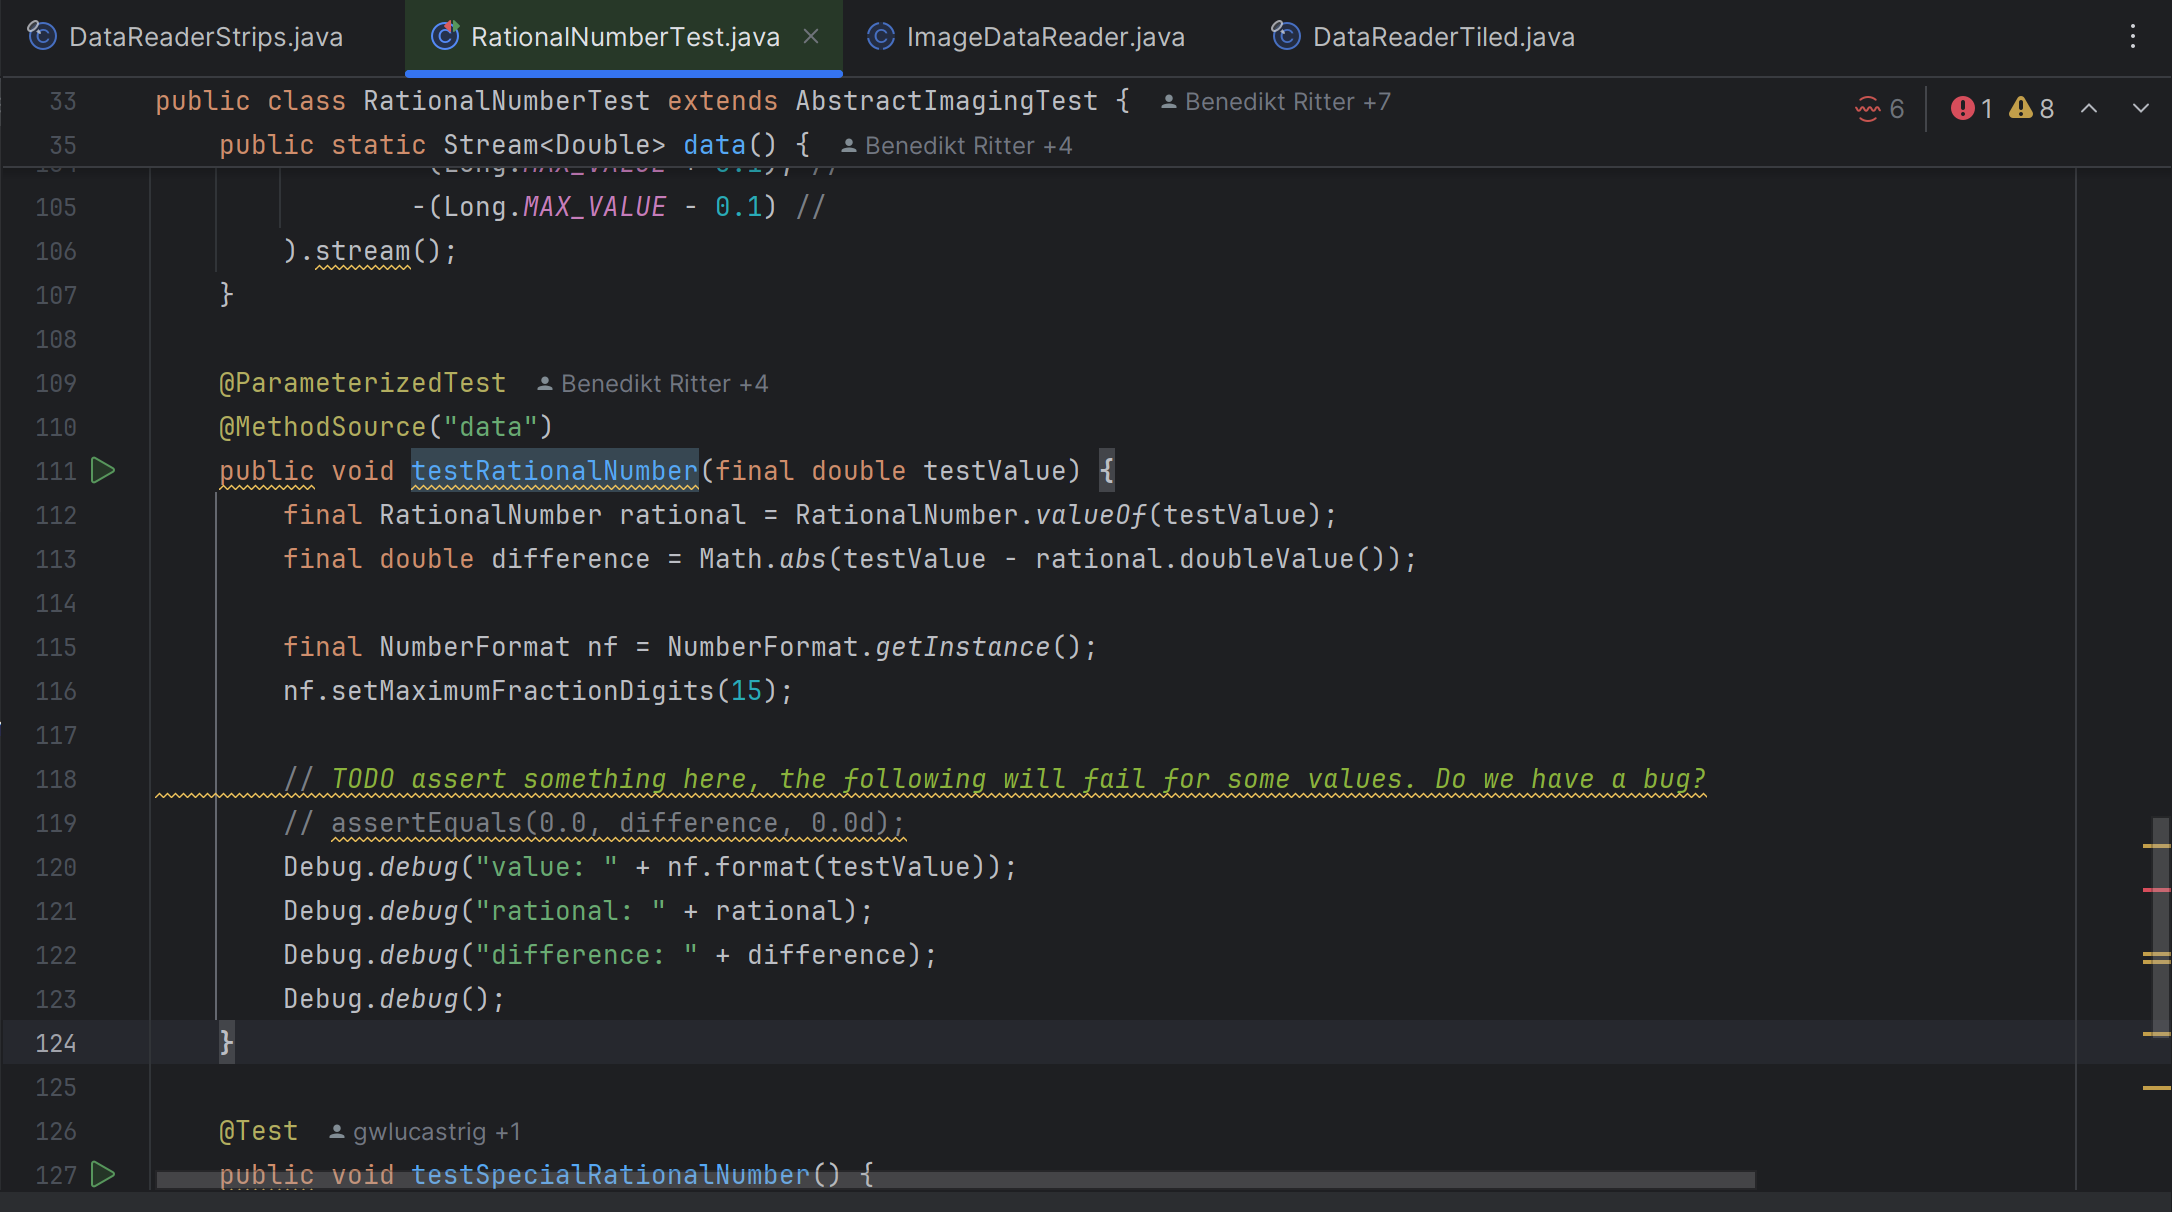
\includegraphics[width=1\textwidth]{Report_Img/assert_issue.png}
    \caption{Example of missing assertions in test cases.}
    \label{fig:assertion_issue}
\end{figure}

\begin{figure}[H]
    \centering
    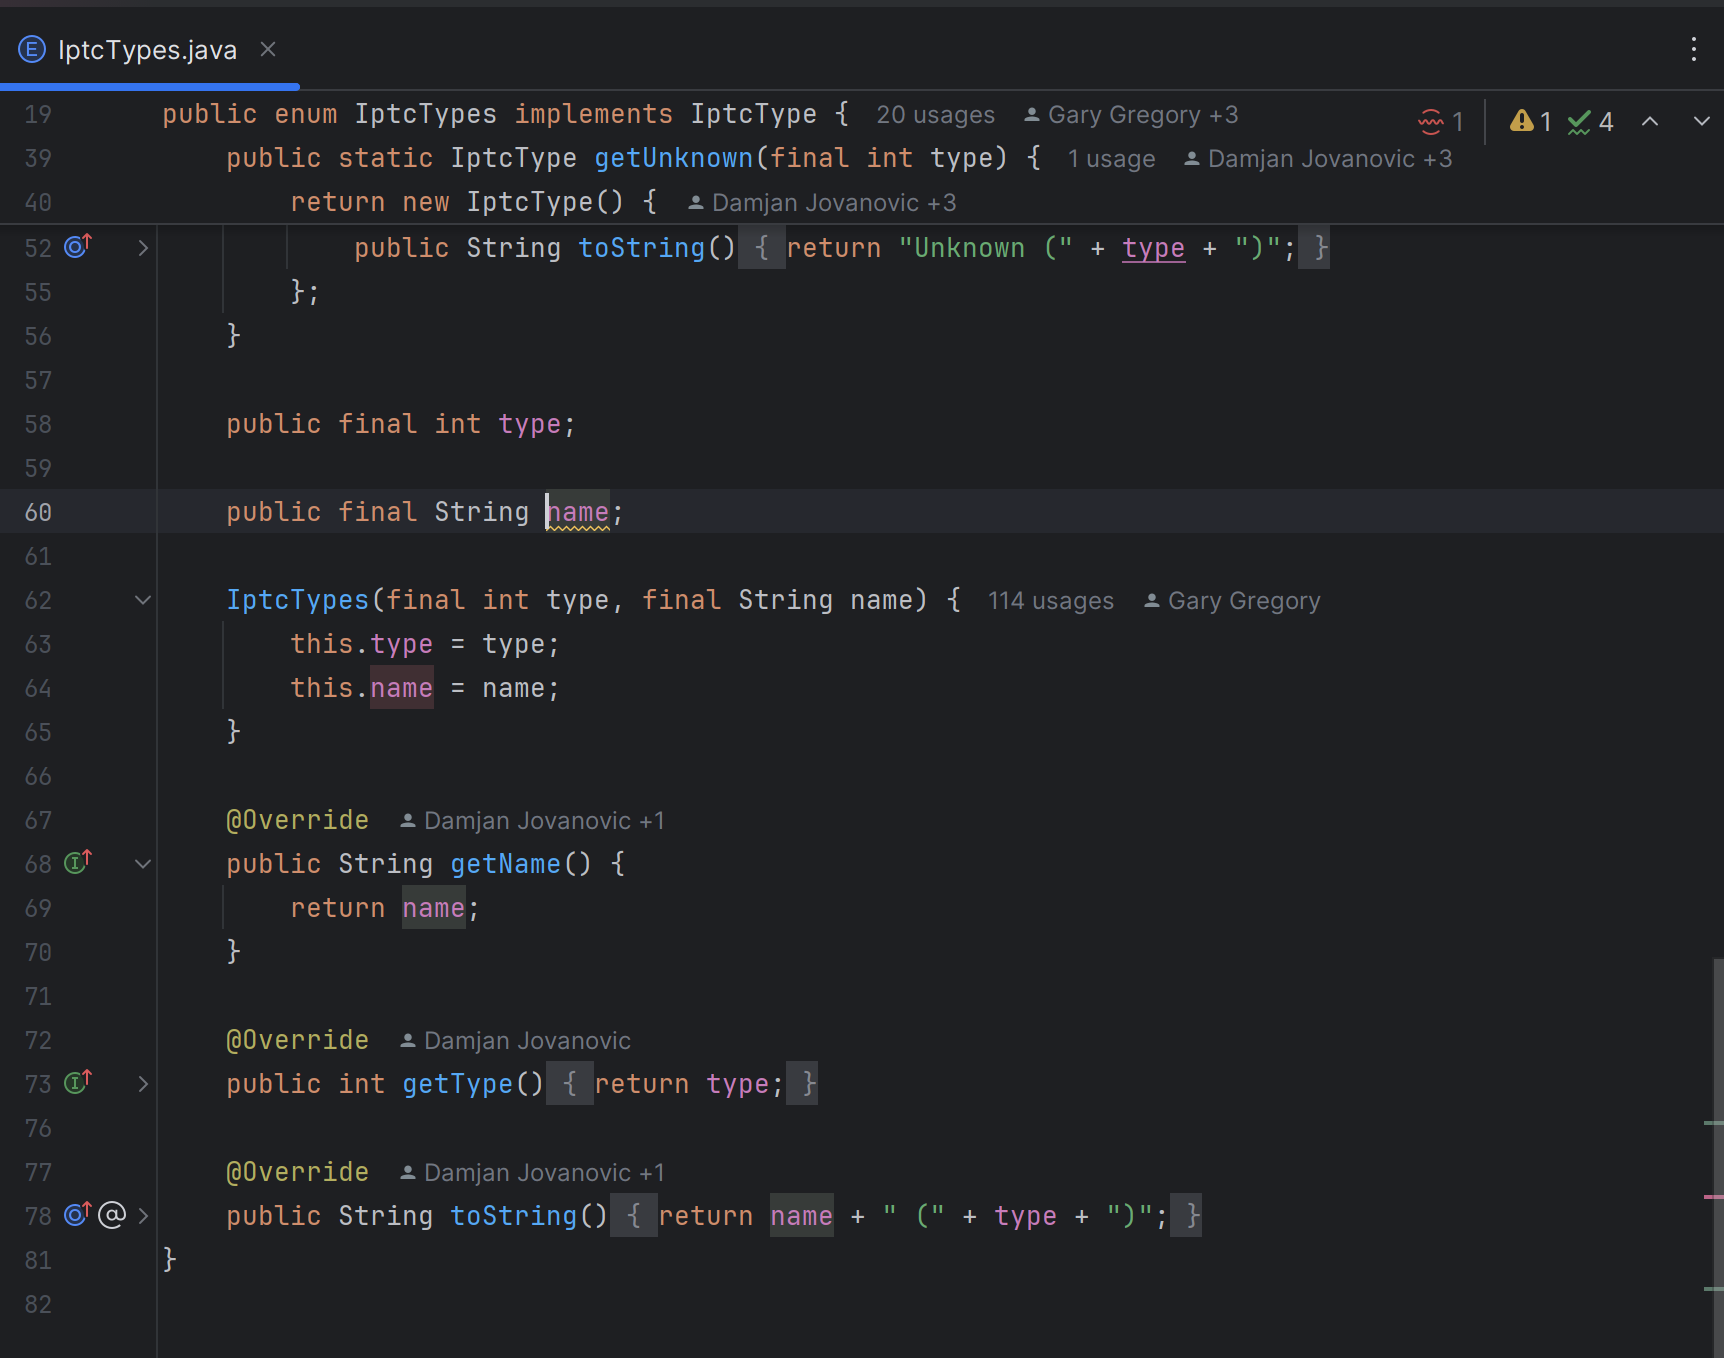
\includegraphics[width=1\textwidth]{Report_Img/naming_issue.png}
    \caption{Example of confusing or duplicate method/variable names.}
    \label{fig:naming_issue}
\end{figure}

\begin{figure}[H]
    \centering
    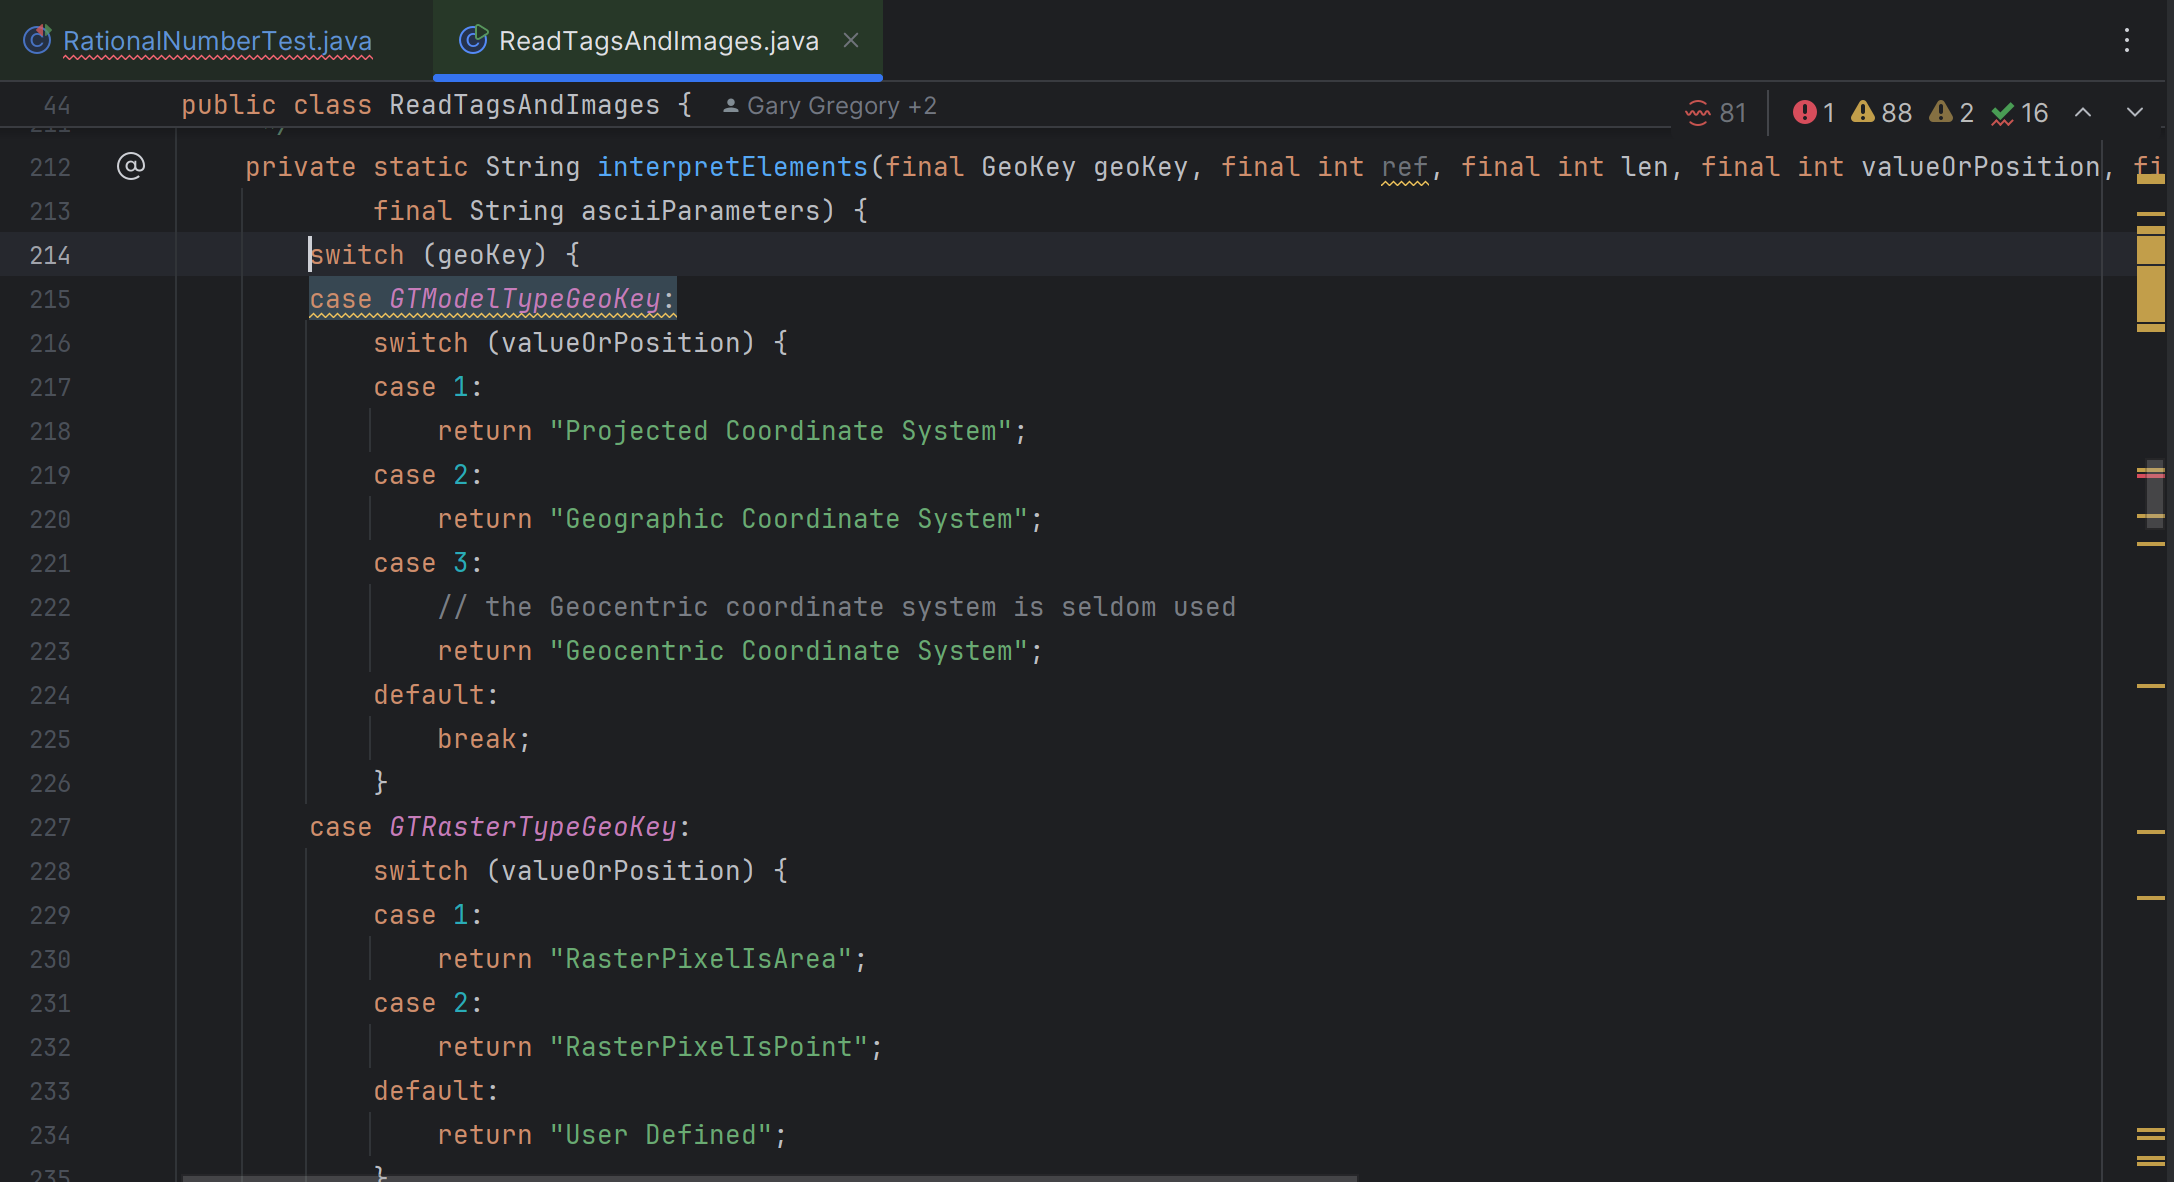
\includegraphics[width=1\textwidth]{Report_Img/break_issue.png}
    \caption{Example of missing break in switch case.}
    \label{fig:missing_break_issue}
\end{figure}

As shown in Figure \ref{fig:fixed_issues}, I successfully resolved 9 issues, but during the process, I also introduced 1 additional issue which is related to commented-out lines of code in the failing test case assertion. This occurred due to a test case that revealed a bug in the code (as noted by the developer). The addition of assertions caused the build process to halt, which is evident in the error log below.

\begin{figure}[H]
    \centering
    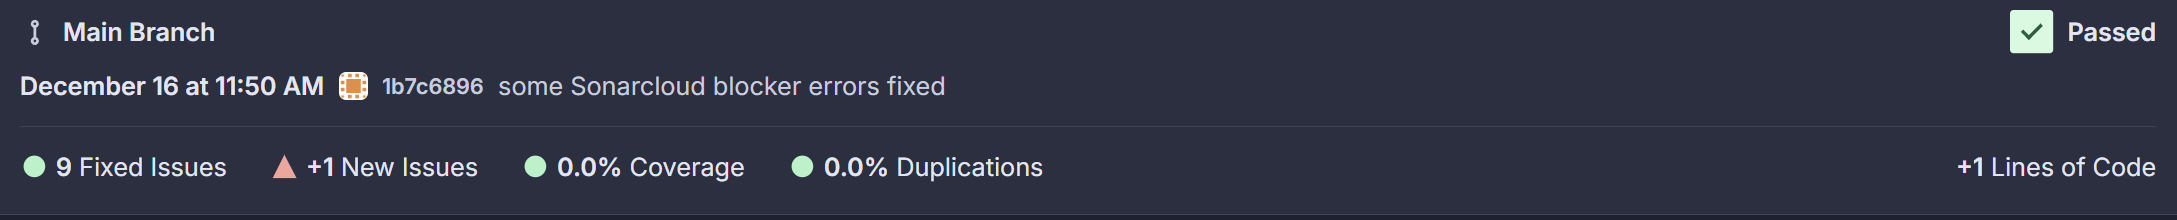
\includegraphics[width=1\textwidth]{Report_Img/issues_fixed.png}
    \caption{9 issues fixed}
    \label{fig:fixed_issues}
\end{figure}

The error message below demonstrates the issue with floating-point precision during the test execution:

\begin{lstlisting}
Assertion Error: \\
[ERROR] Failures: \\
[ERROR]   RationalNumberTest.testRationalNumber:120 The difference between the test value and the rational number representation exceeds the tolerance. \\
       ==> expected: <0.0> but was: <0.0020000040531158447> \\
[INFO] \\
[ERROR] Tests run: 1076, Failures: 15, Errors: 0, Skipped: 7 \\
[INFO] 

Patterns in Failures: \\
Small differences (<1e-9) might be acceptable due to floating-point arithmetic. \\
Large differences (e.g., 0.09999990463256836 or 9.223372034707292E18) are likely bugs or limitations in RationalNumber handling. \\
Therefore, the implementation of \texttt{rationalNumber.valueOf()} must be reviewed by the developer. \\
This problem was tagged as "Accepted" on SonarQube.
\end{lstlisting}

\begin{figure}[H]
    \centering
    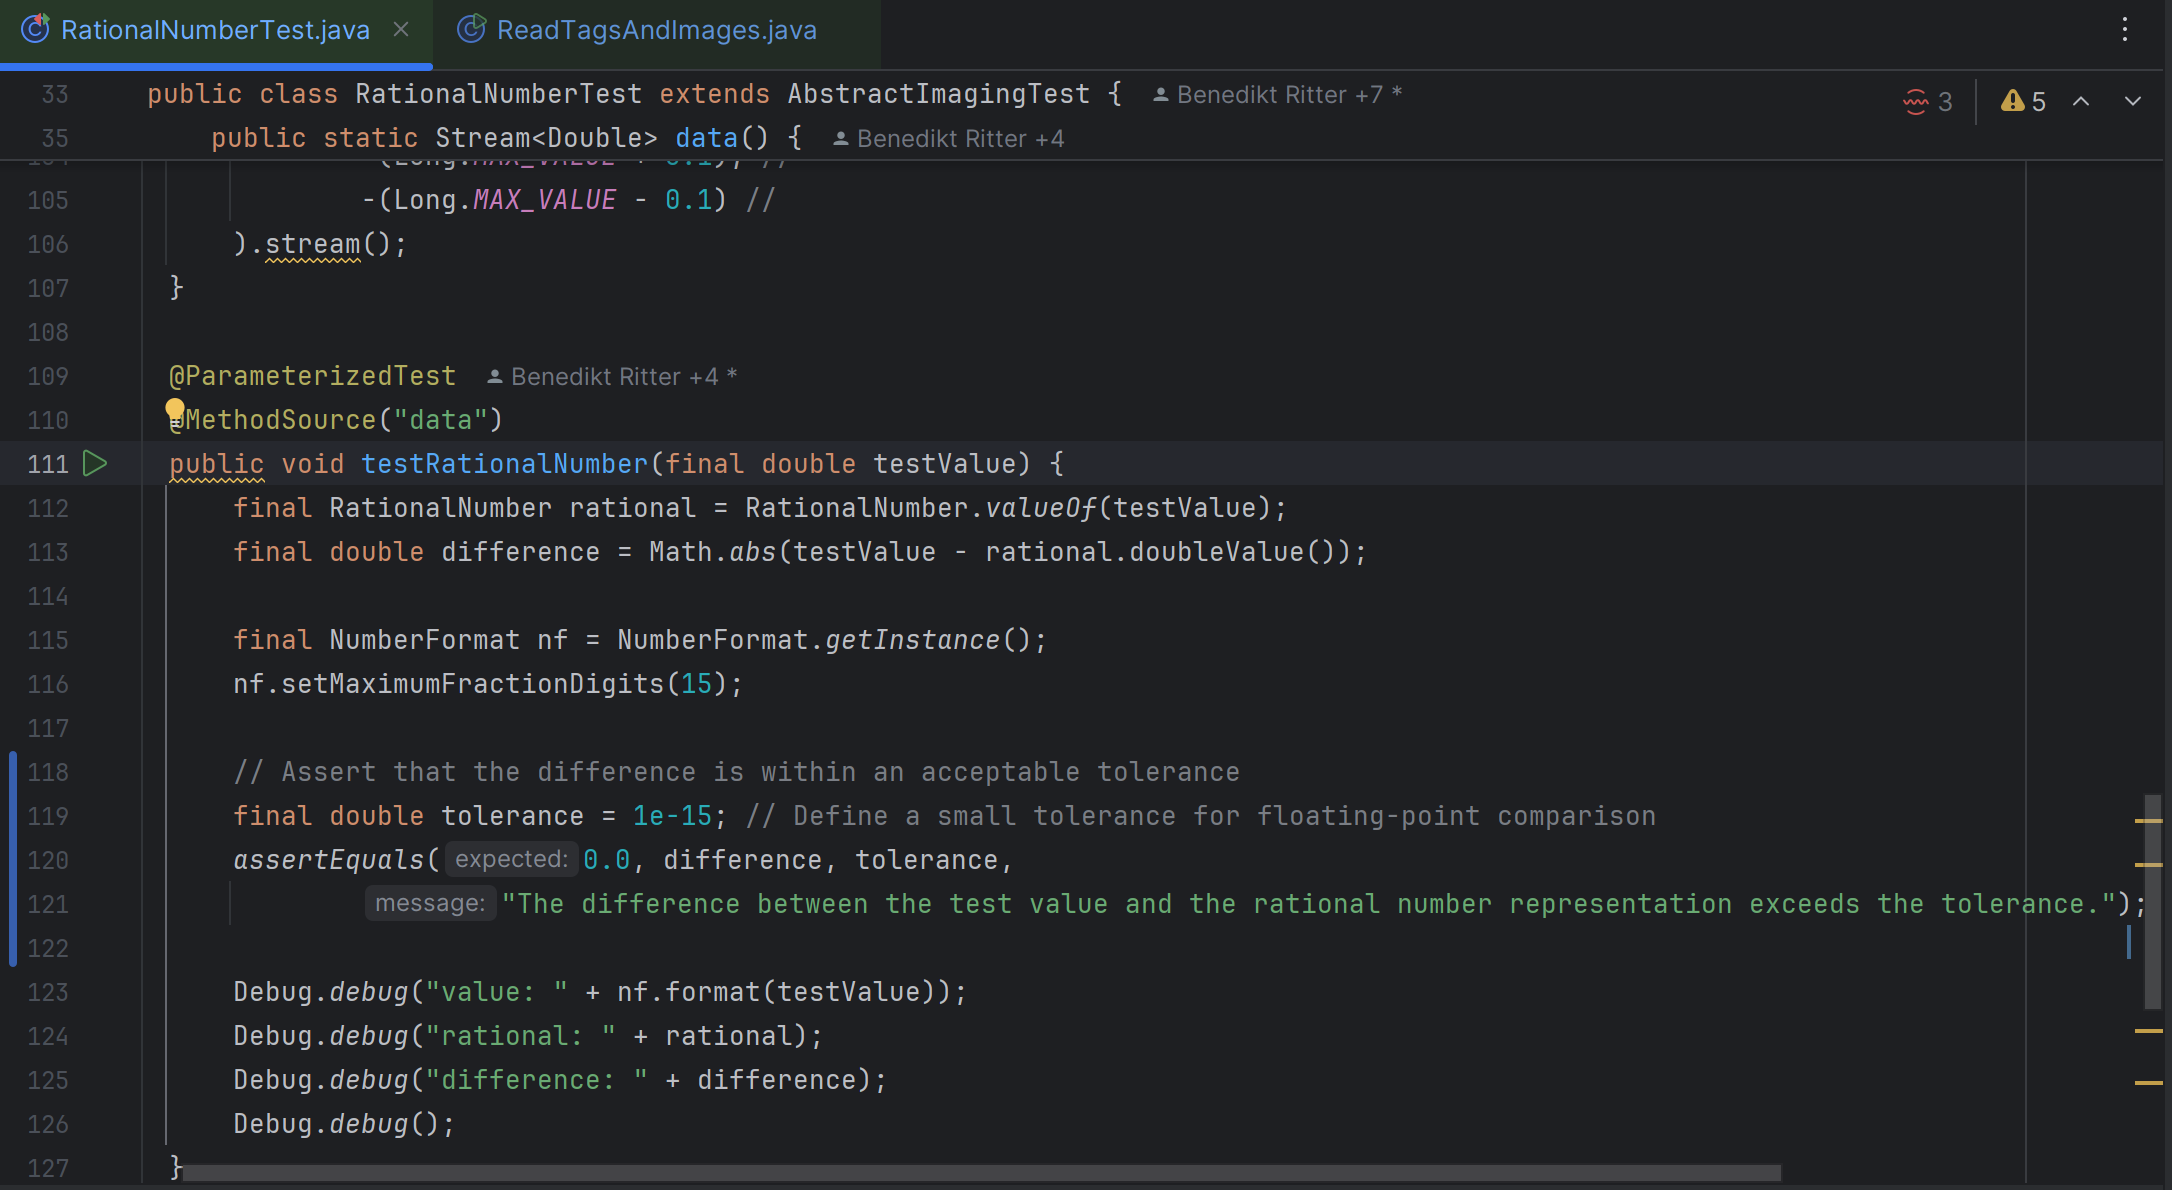
\includegraphics[width=1\textwidth]{Report_Img/assert_fix_error.png}
    \caption{Build halted due to failed assertions and floating-point precision issue of this test case.}
    \label{fig:assertion_error}
\end{figure}

The issues related to floating-point precision need careful attention, as small discrepancies in numerical computations are often acceptable, but larger discrepancies indicate potential bugs. The developer has flagged the issue for further investigation; So I tagged this issue as "Accepted" on SonarQube.
\\
\\
\\
Also in (Figures \ref{fig:unfixable_naming_issue}, \ref{fig:unfixable_naming_issue_accepted}), there is an issue labeled "child class fields should not shadow parent class fields" which is unfixable because the parent class field is a protected variable and cannot be accessed by the child class so any change to both the naming and/or syntax/keywords used for variables could result in an unwanted scenario and/or a bug. So I tagged this issue as "accepted" too.

\begin{figure}[H]
    \centering
    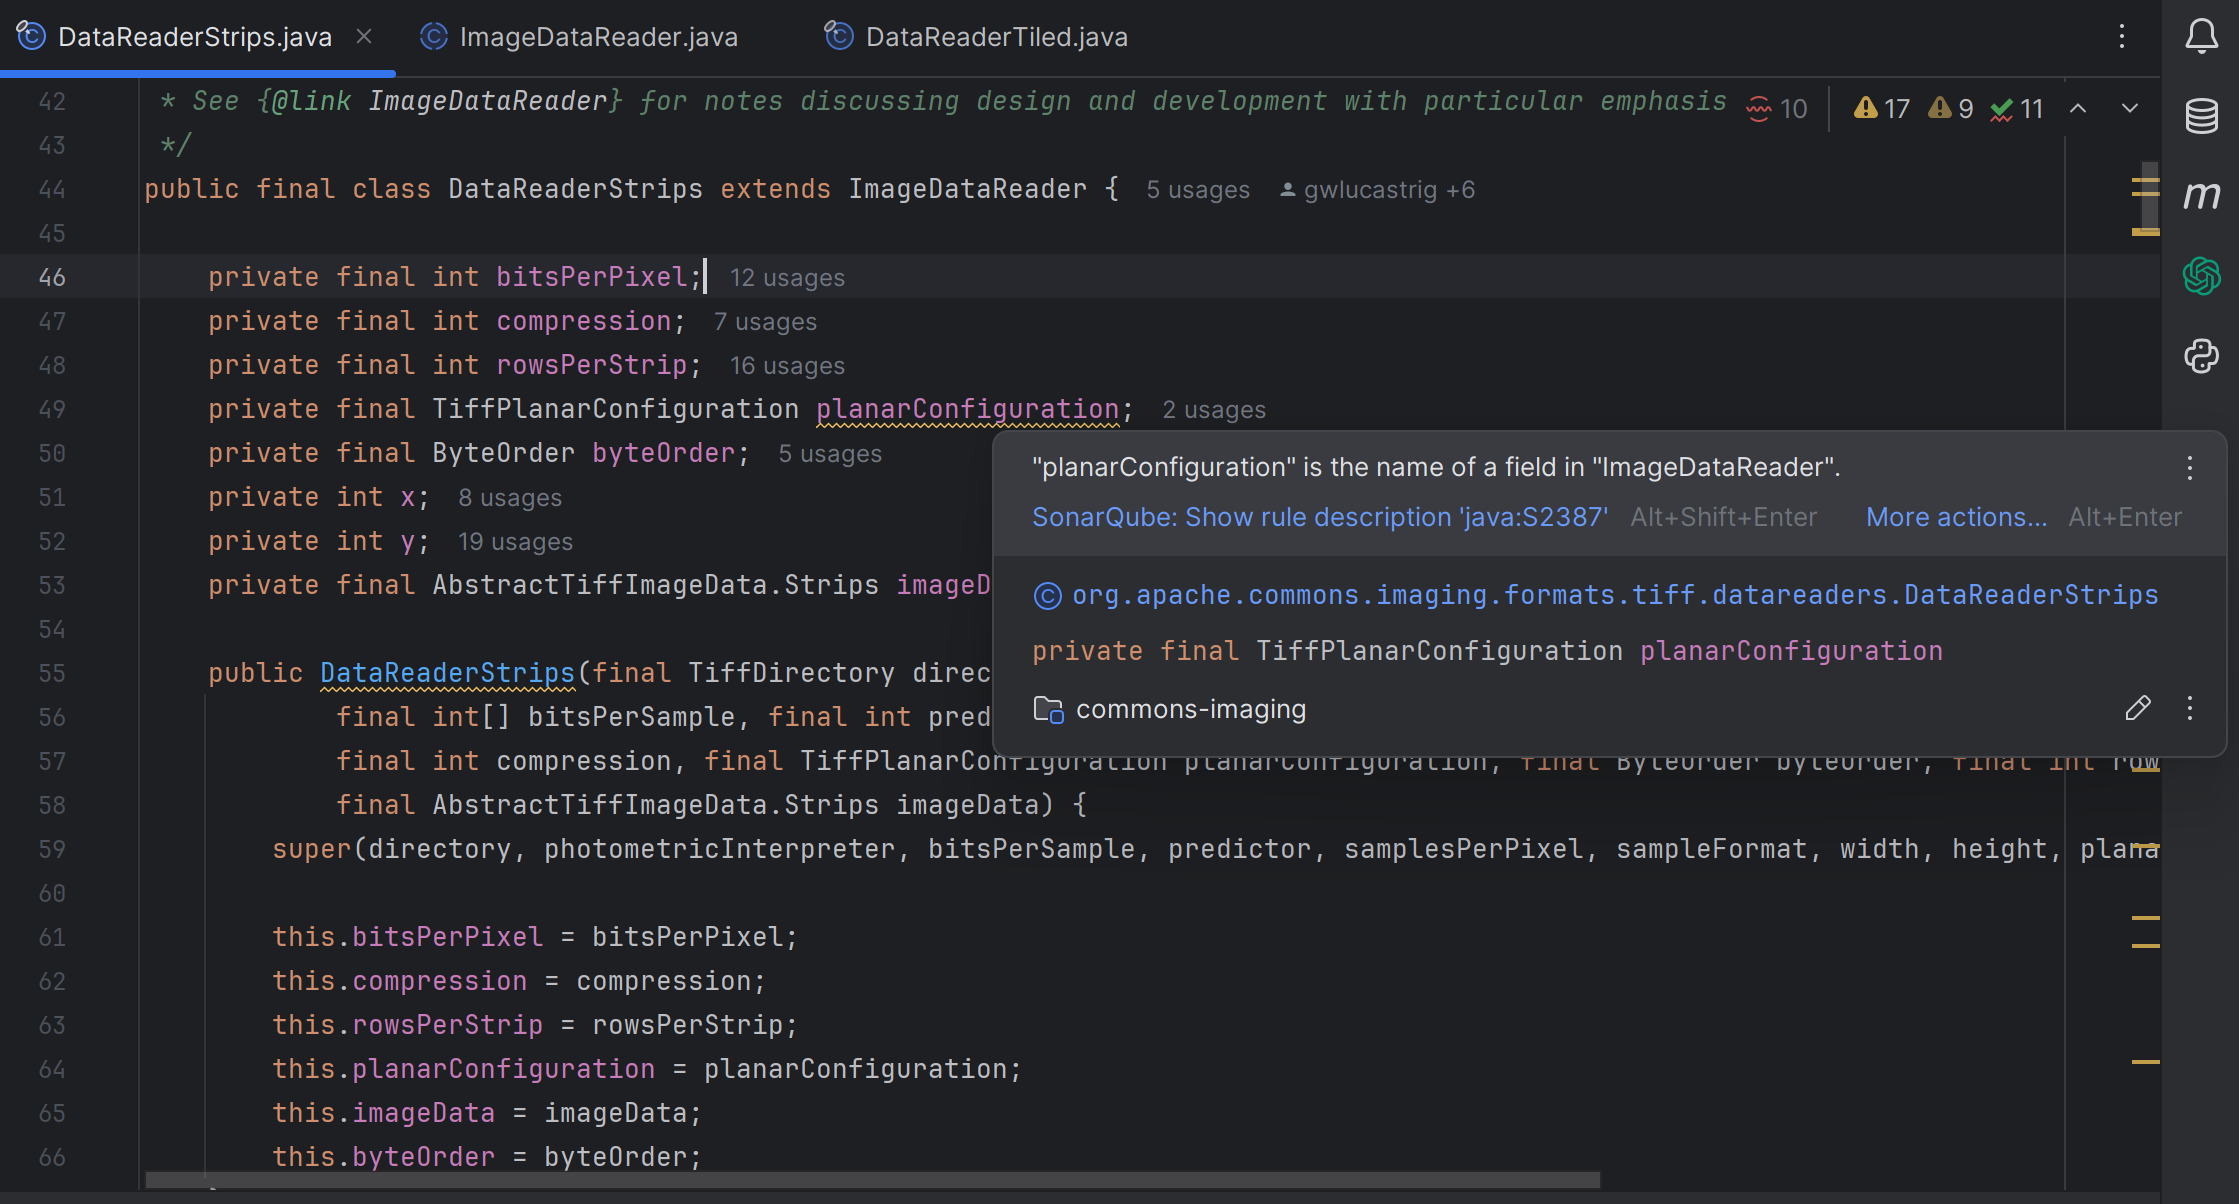
\includegraphics[width=1\textwidth]{Report_Img/unfixable_naming_issue.png}
    \caption{Unfixable naming issue}
    \label{fig:unfixable_naming_issue}
\end{figure}

\begin{figure}[H]
    \centering
    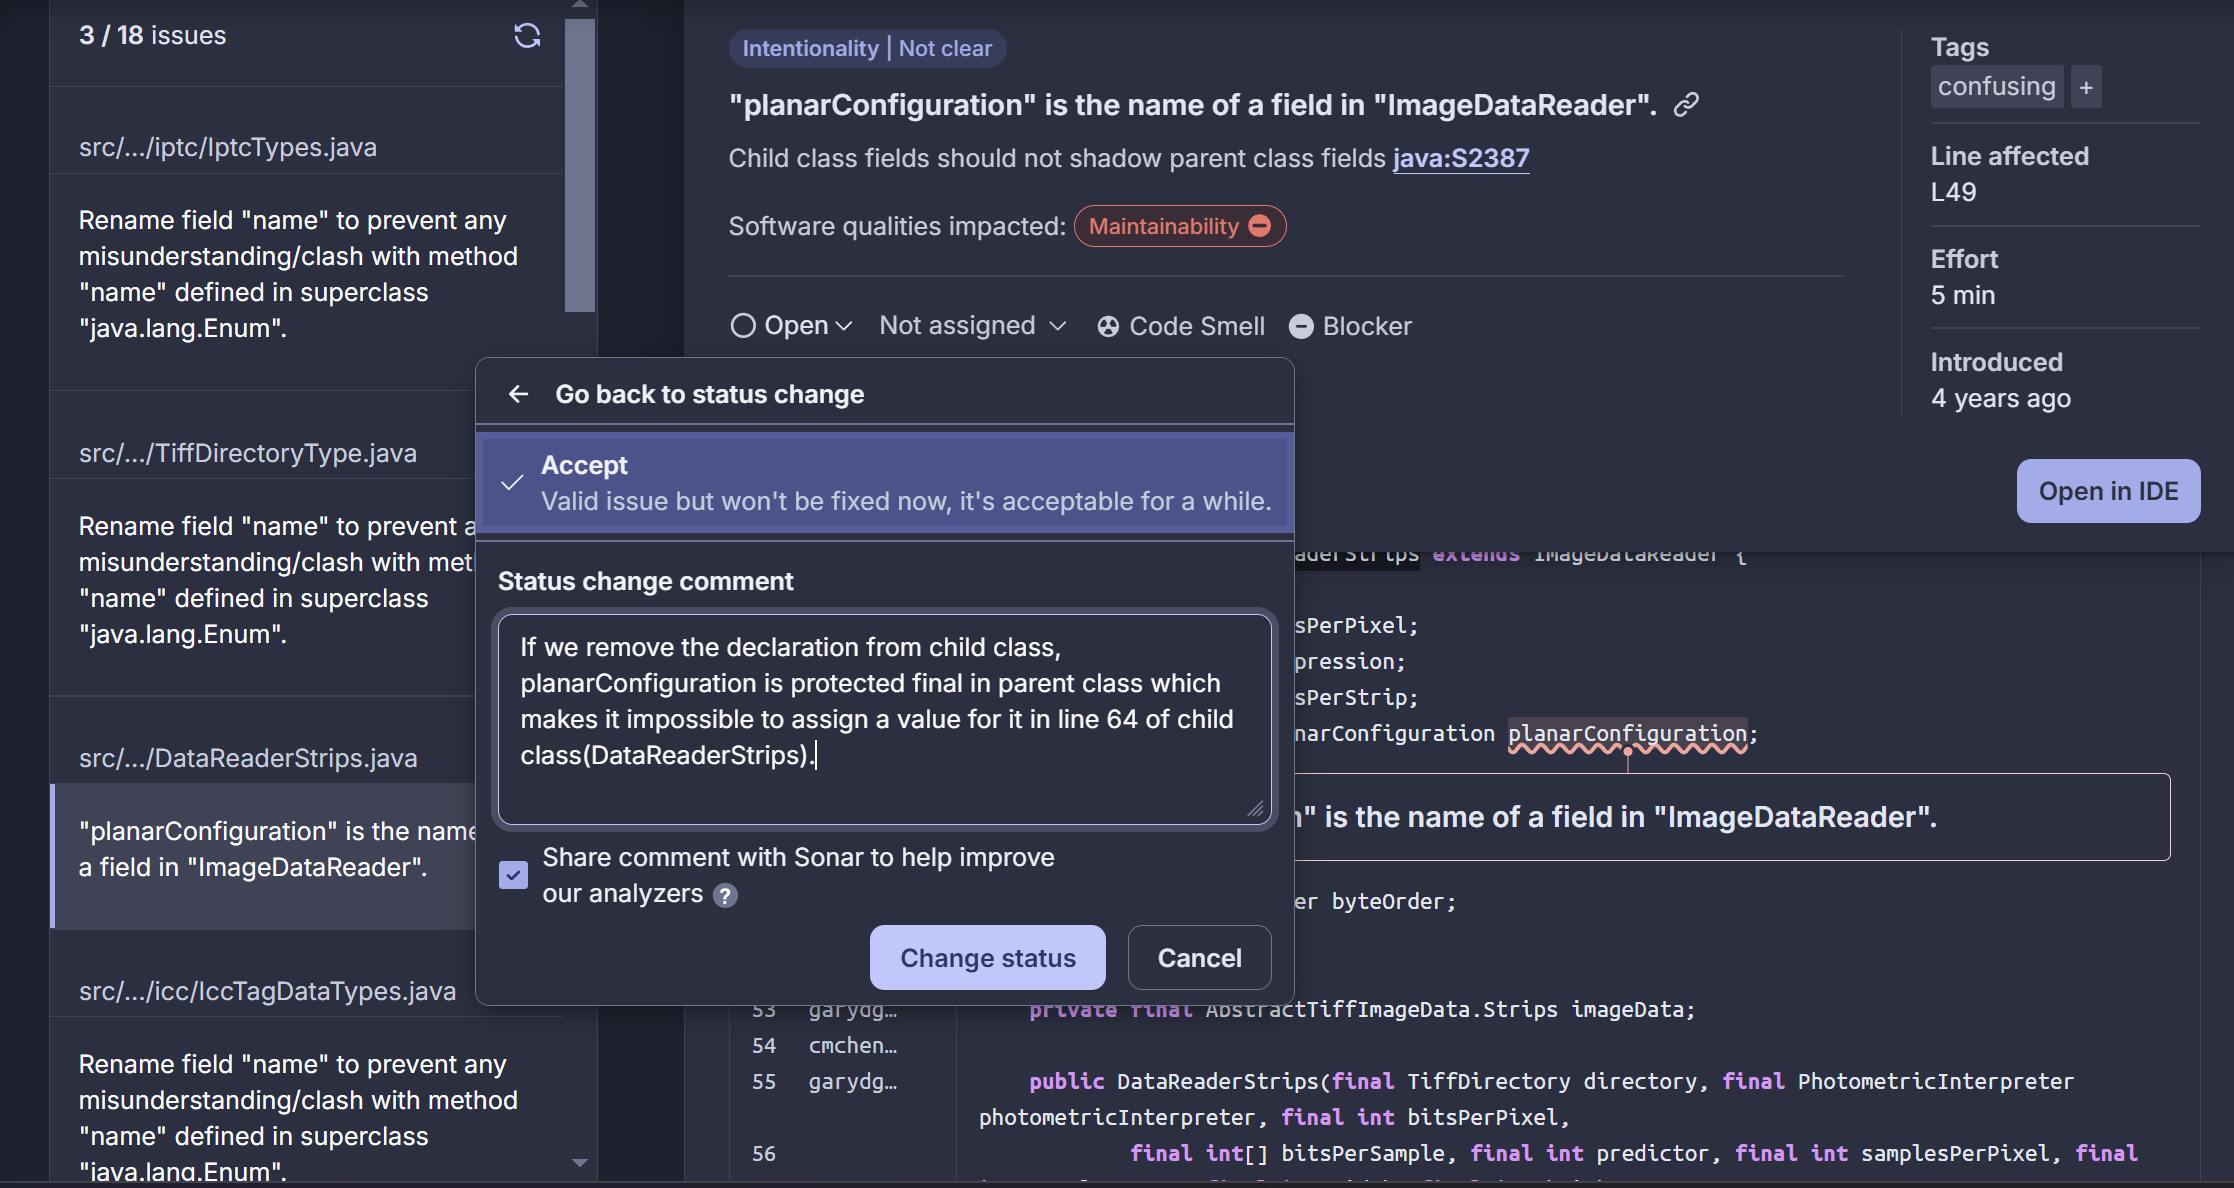
\includegraphics[width=1\textwidth]{Report_Img/unfixable_naming_issue_accepted.png}
    \caption{Unfixable naming issue tagged as "accepted"}
    \label{fig:unfixable_naming_issue_accepted}
\end{figure}












% Docker Image Creation and Containerization
\chapter{Docker Image Creation and Containerization}
The \textit{commons-imaging} project, being an API and utility without a main method, required an additional web application for demonstration purposes. A simple web application was created using React.js for the frontend and Java Spring Boot for the backend. This setup allows the utility to be integrated into a functional system for testing and deployment.

\section{Docker Image and Containerization}
Two Docker images were created for the web application's frontend and backend. These images were pushed to DockerHub and configured to run together using Docker Compose. This ensures seamless orchestration and ease of deployment.

\begin{figure}[H]
    \centering
    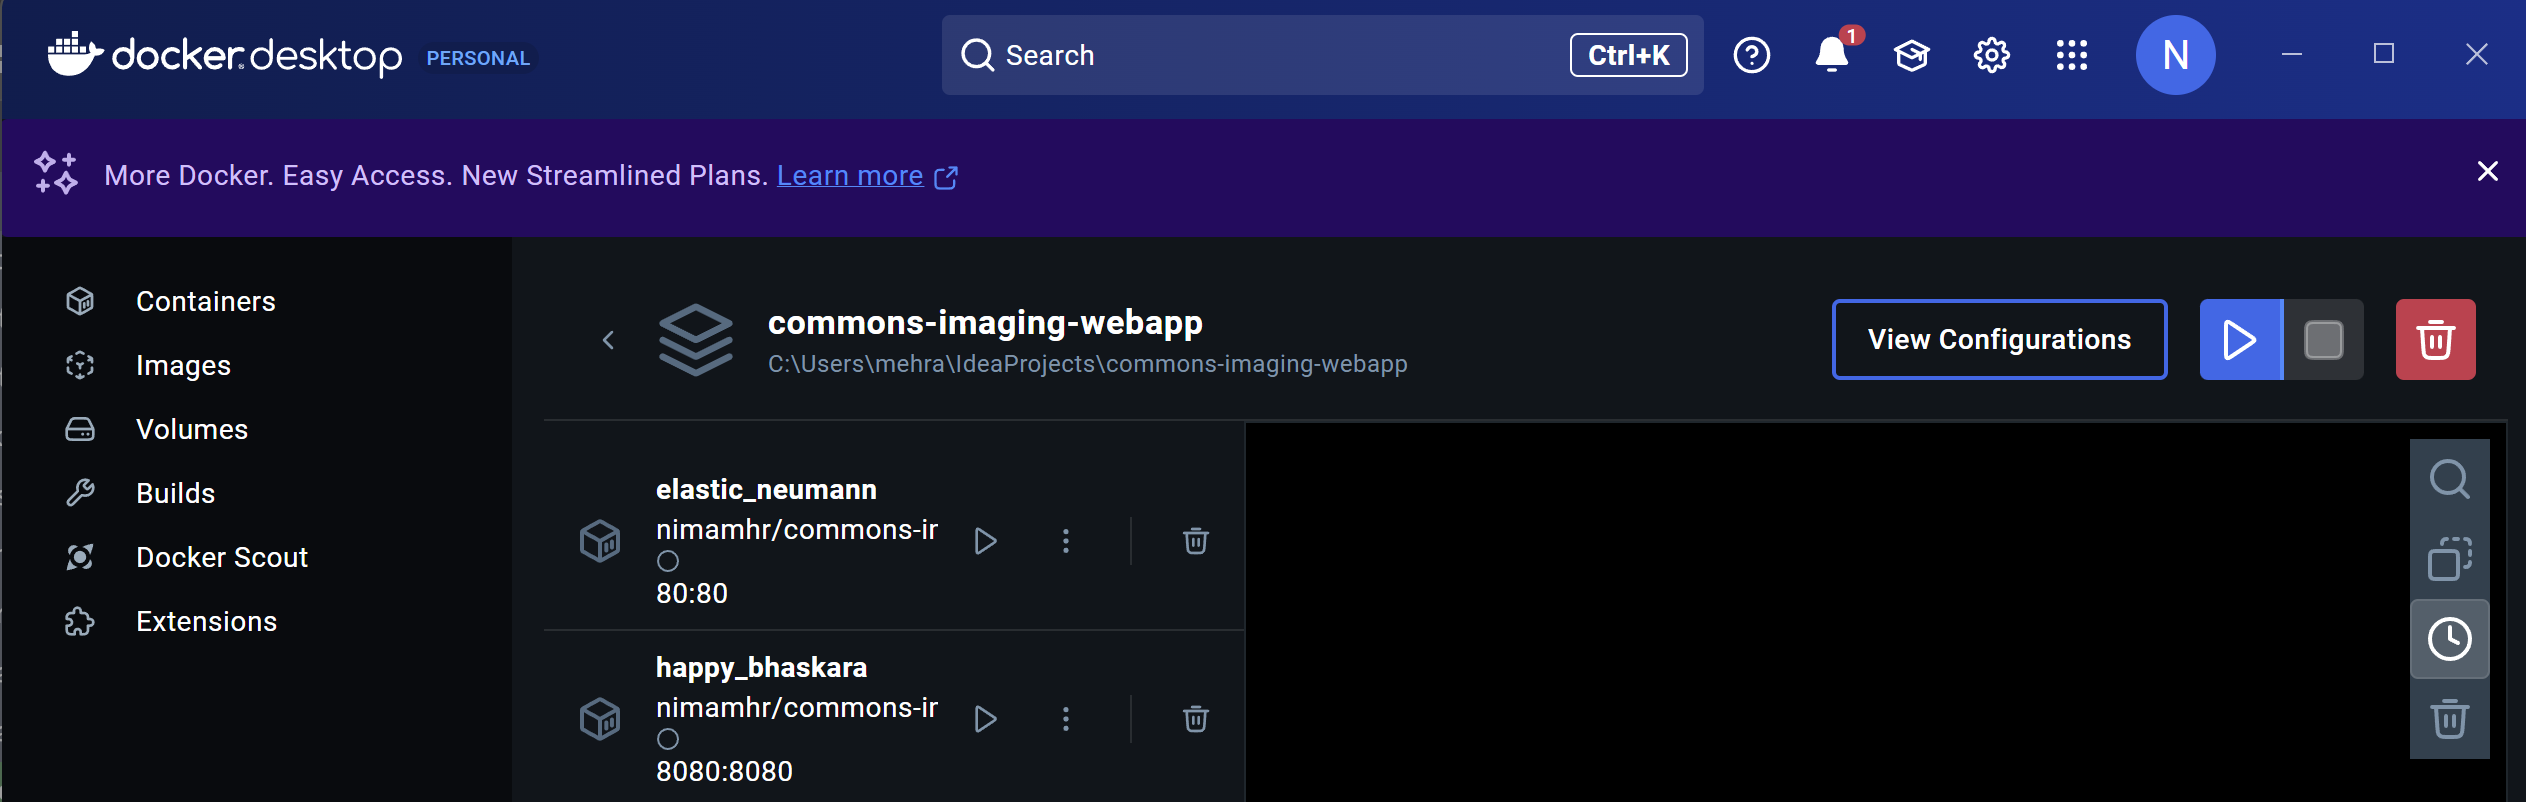
\includegraphics[width=1\textwidth]{Report_Img/docker_desktop.png}
    \caption{Docker Architecture for the commons-imaging-webapp.}
    \label{fig:docker_architecture}
\end{figure}

\section{Dockerfile for Frontend}
The Dockerfile for the frontend builds a React.js application and serves it using Nginx. Below is the configuration:

\begin{lstlisting}[language=dockerfile, caption=Dockerfile for commons-imaging-webapp Frontend]
FROM node:18-alpine AS build
WORKDIR /app
COPY package.json package-lock.json ./
RUN npm install
COPY . ./
RUN npm run build
FROM nginx:alpine
COPY --from=build /app/build /usr/share/nginx/html
EXPOSE 80
CMD ["nginx", "-g", "daemon off;"]
\end{lstlisting}

\section{Dockerfile for Backend}
The backend is a Java Spring Boot application. The Dockerfile compiles the application and creates an executable JAR file:

\begin{lstlisting}[language=dockerfile, caption=Dockerfile for commons-imaging-webapp Backend]
FROM openjdk:24-jdk
WORKDIR /app
COPY .mvn/ .mvn
COPY mvnw pom.xml ./
RUN ./mvnw dependency:go-offline -B
COPY src/ ./src
RUN ./mvnw clean package -DskipTests
EXPOSE 8080
CMD ["java", "-jar", "target/test-0.0.1-SNAPSHOT.jar"]
\end{lstlisting}

\section{Docker Compose Configuration}
The Docker Compose file orchestrates both the frontend and backend services, setting up a shared network and dependencies.

\begin{lstlisting}[language=dockerfile, caption=Docker Compose File for Orchestration]
version: '3.7'

services:
  backend:
    build:
      context: ./Backend
    ports:
      - "8080:8080"
    networks:
      - app-network

  frontend:
    build:
      context: ./commons-imaging-test
    ports:
      - "80:80"
    environment:
      - REACT_APP_API_URL=http://backend:8080  # API URL for backend
    networks:
      - app-network
    depends_on:
      - backend

networks:
  app-network:
    driver: bridge
\end{lstlisting}

\section{DockerHub Synchronization}
The Docker images for both the frontend and backend are synchronized with DockerHub for easy access. They can be pulled and run using the following commands:
\newpage
\subsection{Pulling Docker Images}
\begin{lstlisting}[language=bash, caption=Pull Docker Images from DockerHub]
docker pull nimamhr/commons-imaging-webapp-frontend:latest
docker pull nimamhr/commons-imaging-webapp-backend:latest
\end{lstlisting}

\subsection{Running Docker Images}
\begin{lstlisting}[language=bash, caption=Run Docker Images]
docker run -d -p 8080:8080 nimamhr/commons-imaging-webapp-backend:latest
docker run -d -p 80:80 nimamhr/commons-imaging-webapp-frontend:latest
\end{lstlisting}

\subsection{Accessing the Web Application}
Once the containers are running, the web application can be accessed at:\\
\url{http://localhost/}

\begin{figure}[H]
    \centering
    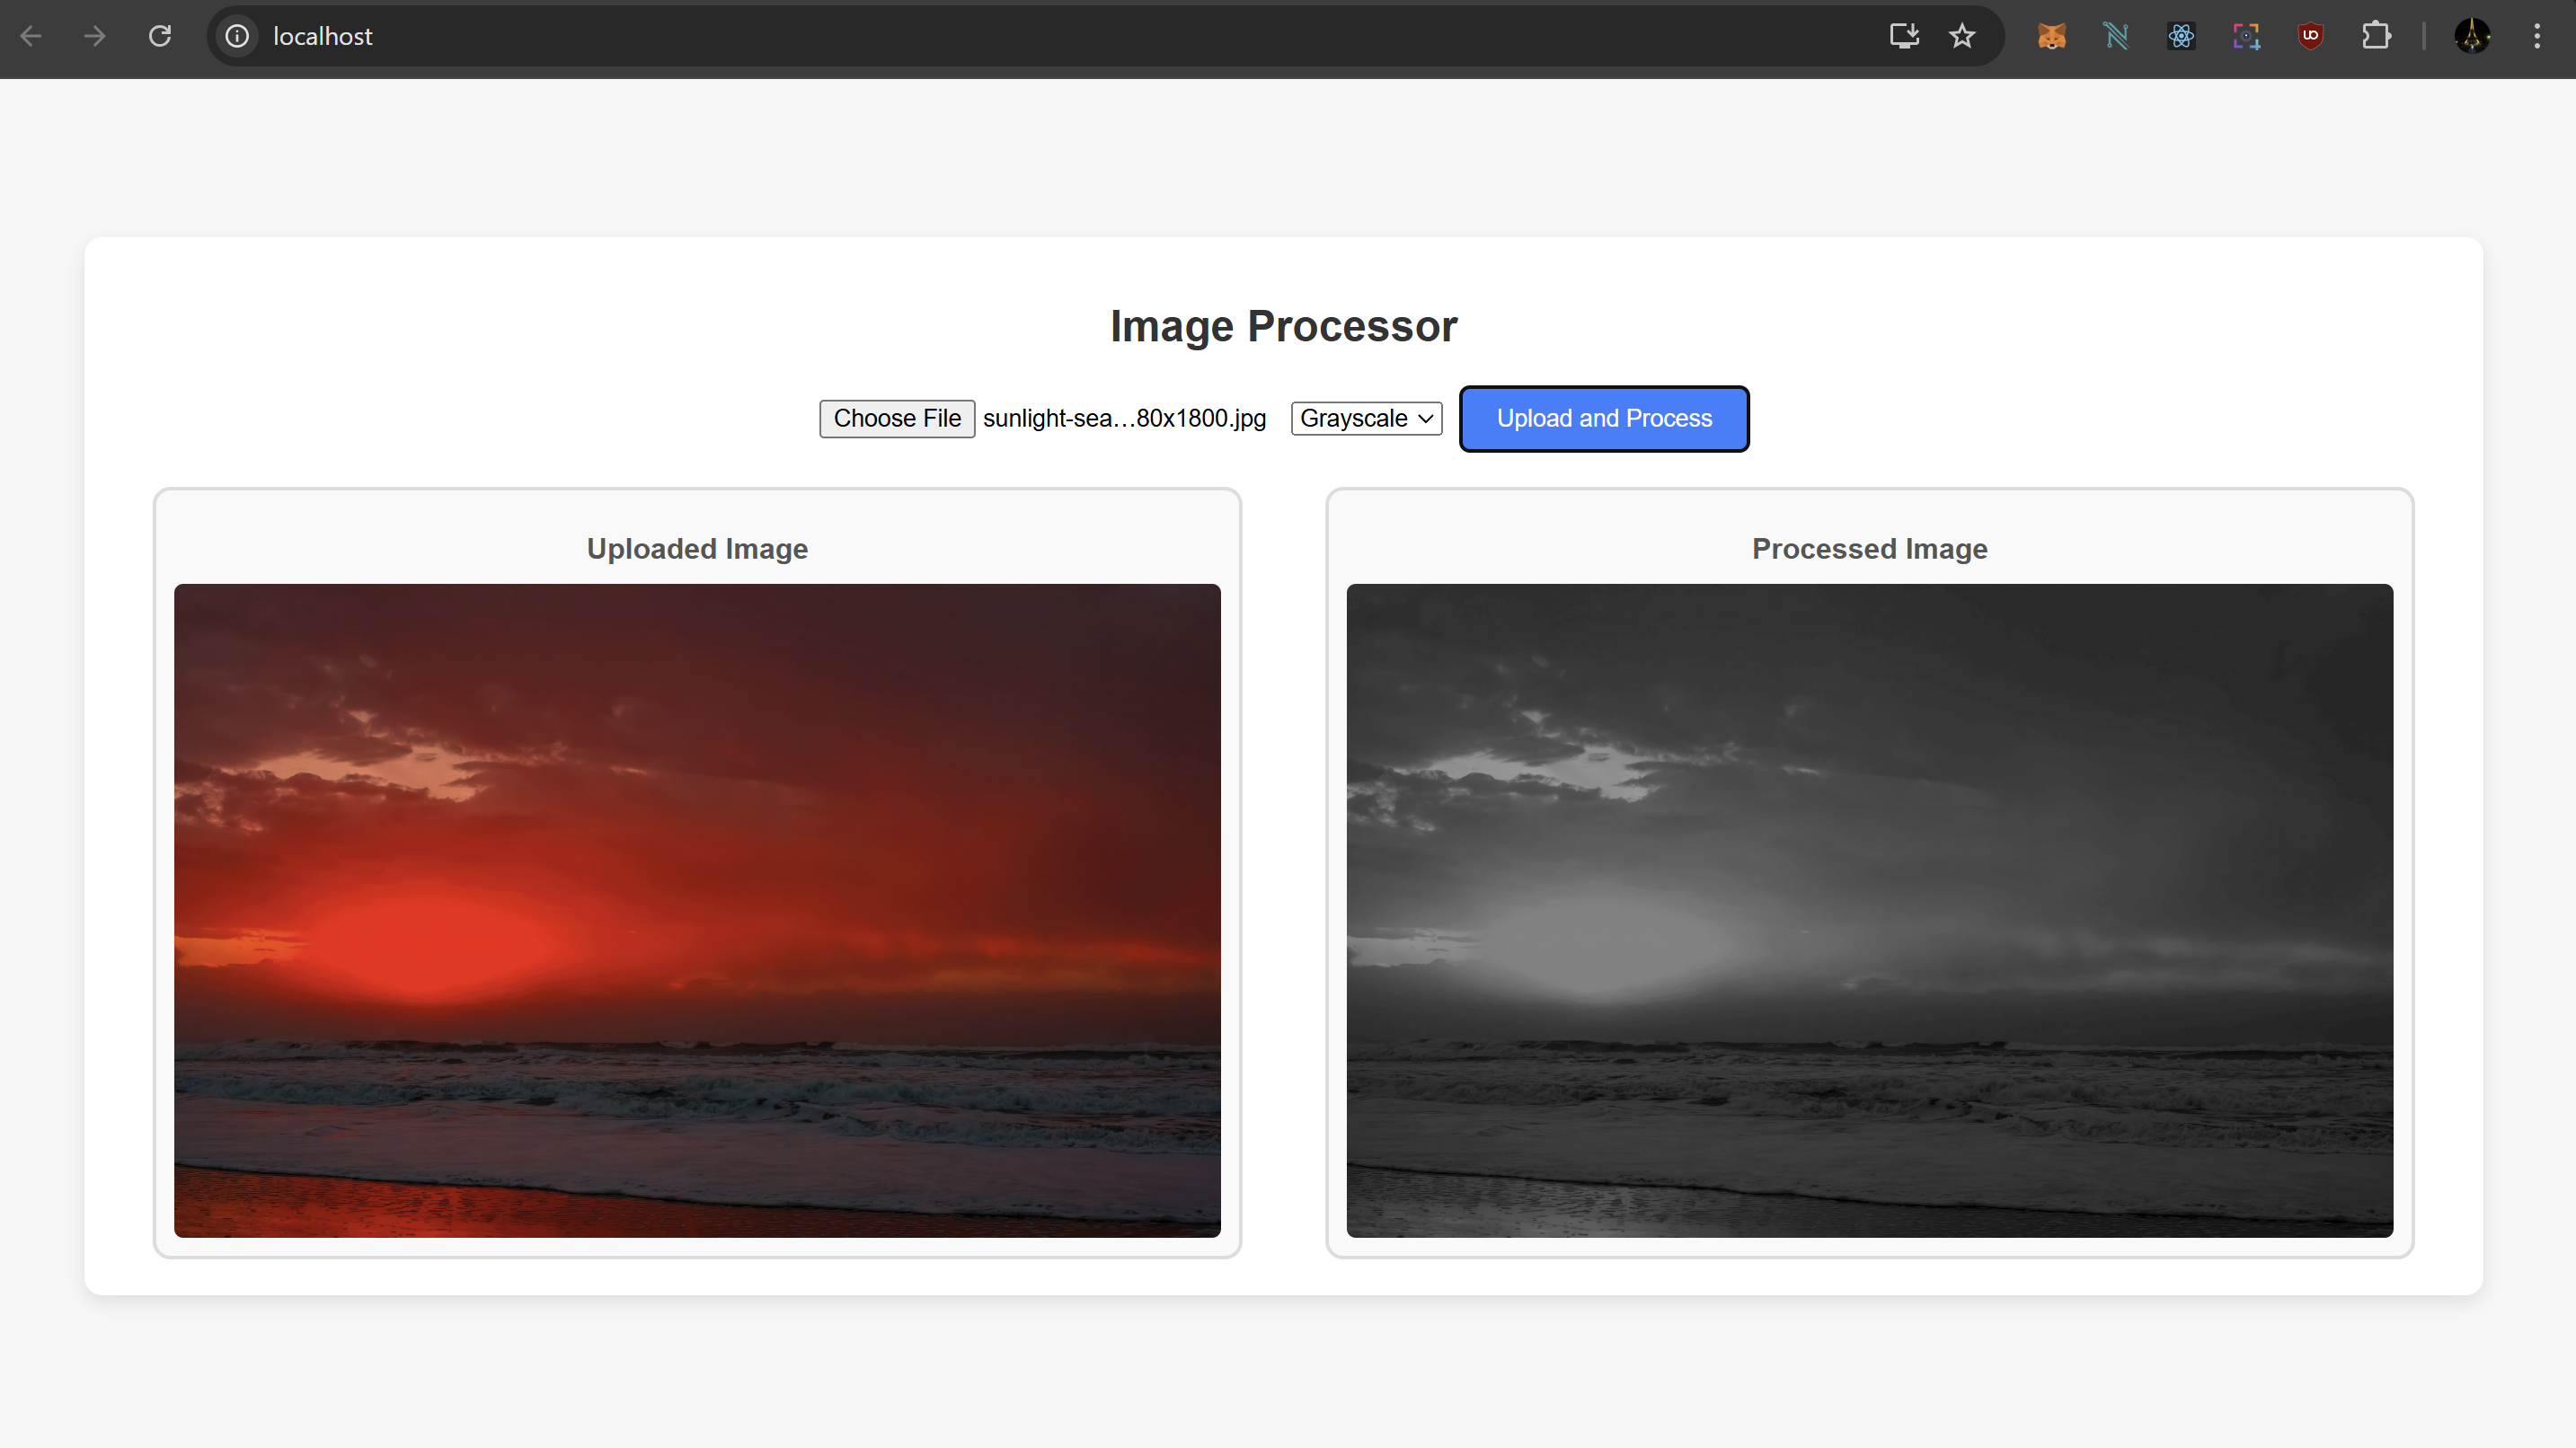
\includegraphics[width=1\textwidth]{Report_Img/localhost.png}
    \caption{Commons-Imaging Test Web Application Interface.}
    \label{fig:webapp_interface}
\end{figure}


% Code Coverage Analysis
\chapter{Code Coverage Analysis}
Code coverage analysis was performed using JaCoCo to assess the extent of test coverage within the \textit{commons-imaging} project. This analysis helped identify untested or poorly tested portions of the codebase, guiding the addition of manual and automated tests.

\section{Setting Up JaCoCo}
To set up JaCoCo for the project, the JaCoCo Maven plugin was added to the \texttt{pom.xml} file. The following commands were then executed to generate code coverage reports:

\begin{lstlisting}[language=bash, caption=Commands to Generate Code Coverage Reports]
mvn clean test
mvn clean verify
\end{lstlisting}

\section{Initial Coverage Results}
The initial code coverage results, before adding tests, are summarized below:

\begin{table}[H]
    \centering
    \begin{tabular}{|l|c|c|c|c|}
        \hline
        \textbf{Element} & \textbf{Missed Instructions} & \textbf{I. Cov. (\%)} & \textbf{Missed Branches} & \textbf{B. Cov. (\%)} \\ \hline
        Total & 21,380 of 95,452 & 77\% & 2,570 of 7,199 & 64\% \\ \hline
    \end{tabular}
    \caption{Initial Code Coverage Results.}
    \label{tab:initial_coverage}
\end{table}

\begin{figure}[H]
    \centering
    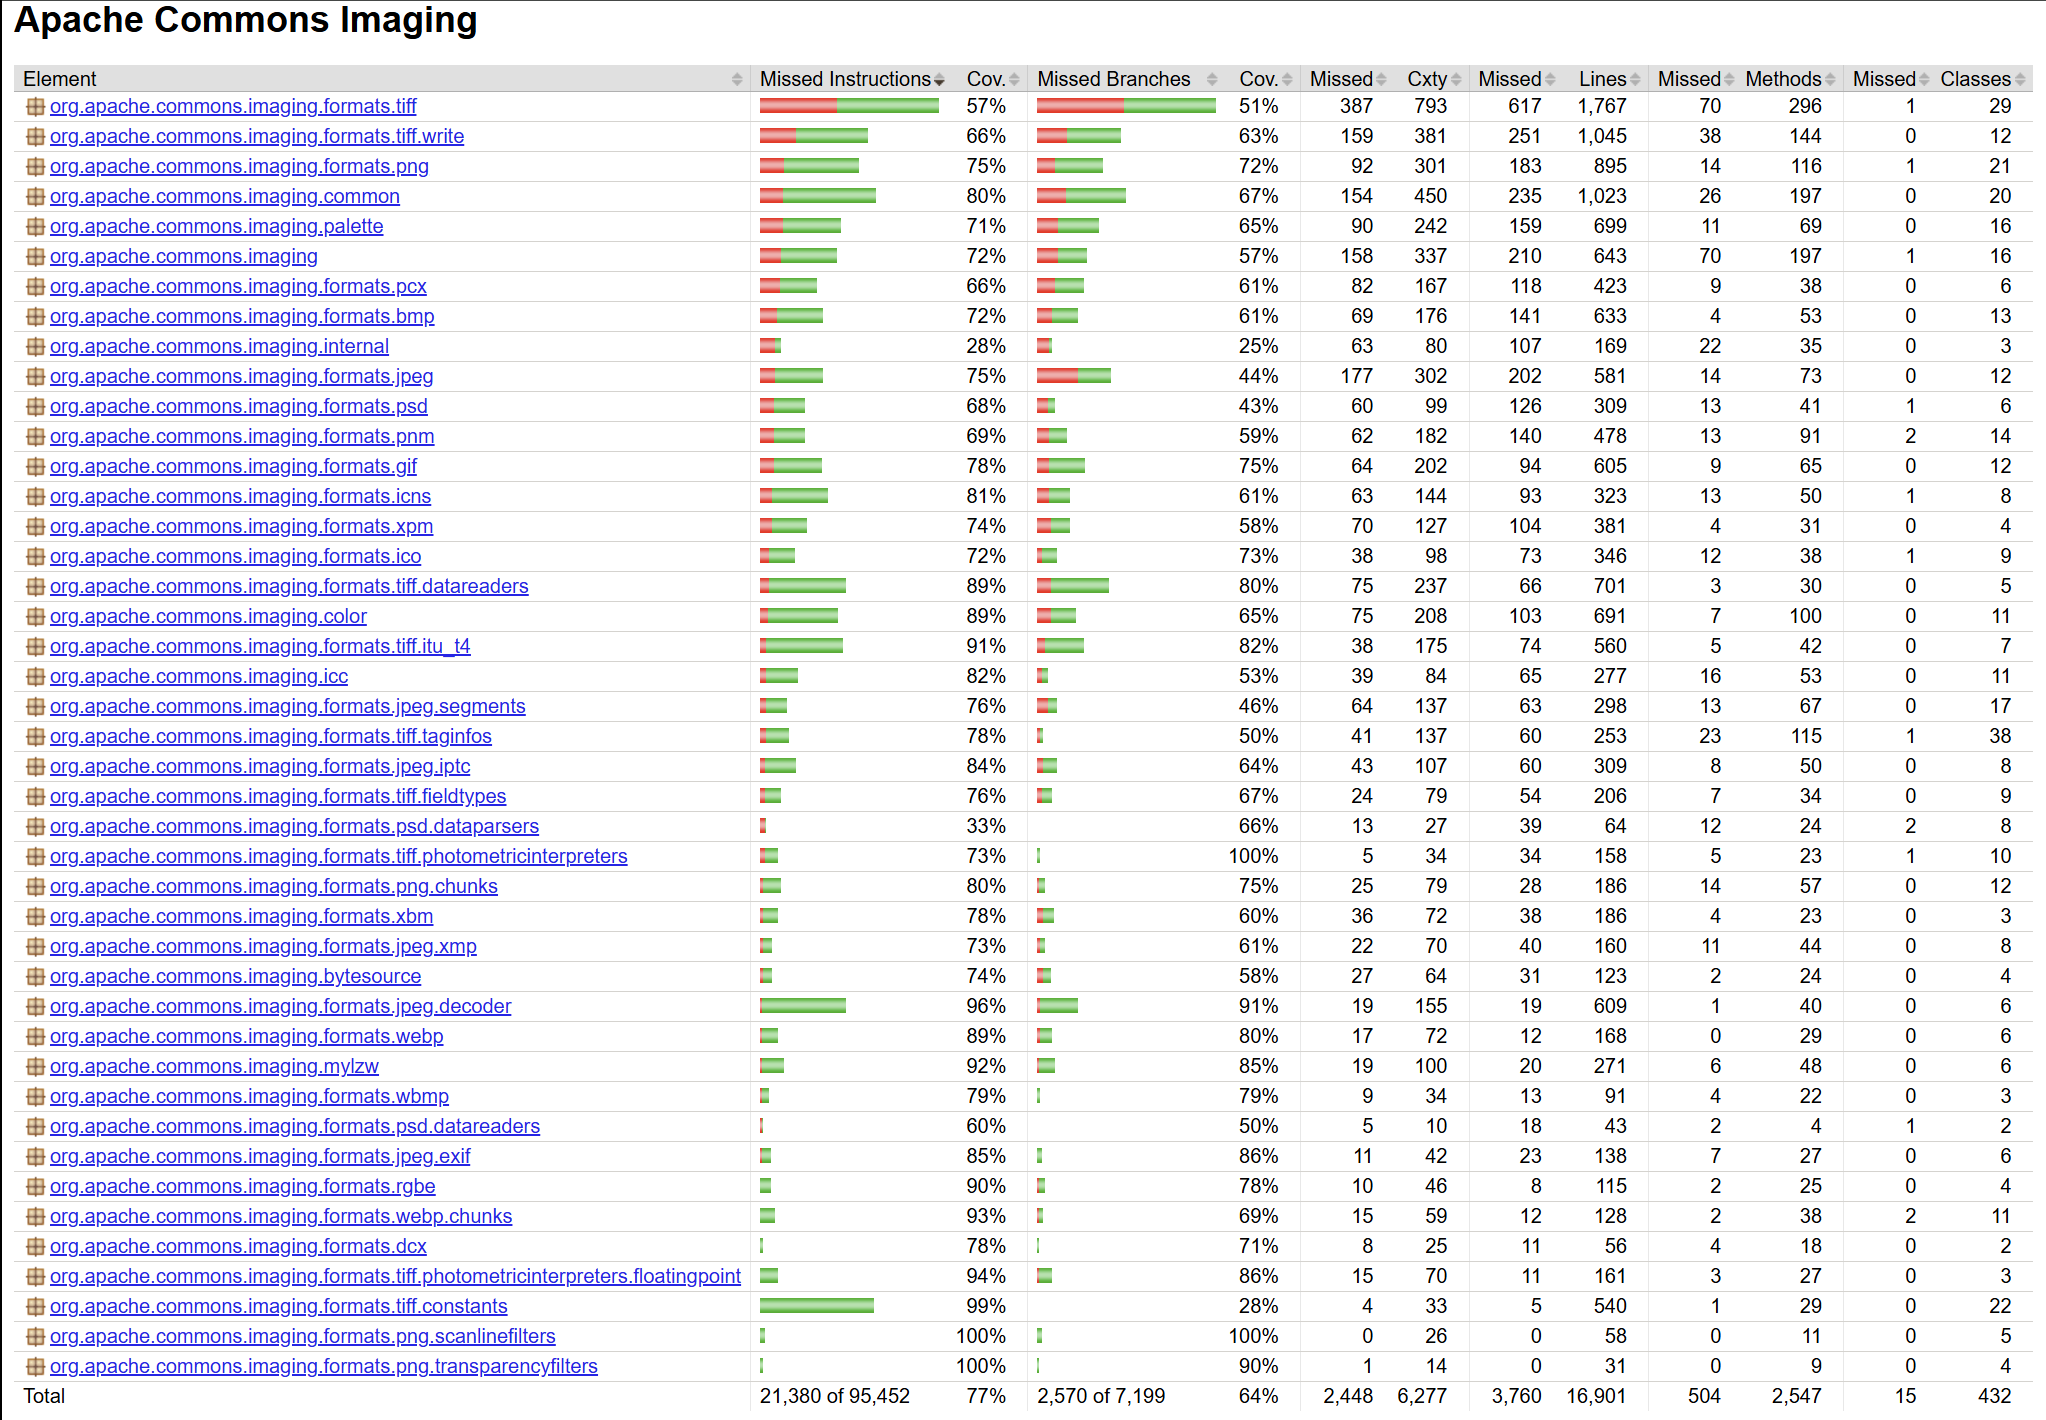
\includegraphics[width=1\textwidth]{Report_Img/init_cov.png}
    \caption{Visualization of Initial Code Coverage Results.}
    \label{fig:initial_coverage_visualization}
\end{figure}
\newpage
\section{Final Coverage Results After Test Improvements}
After generating additional tests using automated tools and adding manual test cases (details are in chapters 6 \& 8), the code coverage improved. The final coverage results are summarized below:

\begin{table}[H]
    \centering
    \begin{tabular}{|l|c|c|c|c|}
        \hline
        \textbf{Element} & \textbf{Missed Instructions} & \textbf{I. Cov. (\%)} & \textbf{Missed Branches} & \textbf{B. Cov. (\%)} \\ \hline
        Total & 18,077 of 95,452 & 81\% & 2,327 of 7,199 & 67\% \\ \hline
    \end{tabular}
    \caption{Final Code Coverage Results After Test Improvements.}
    \label{tab:final_coverage}
\end{table}

\begin{figure}[H]
    \centering
    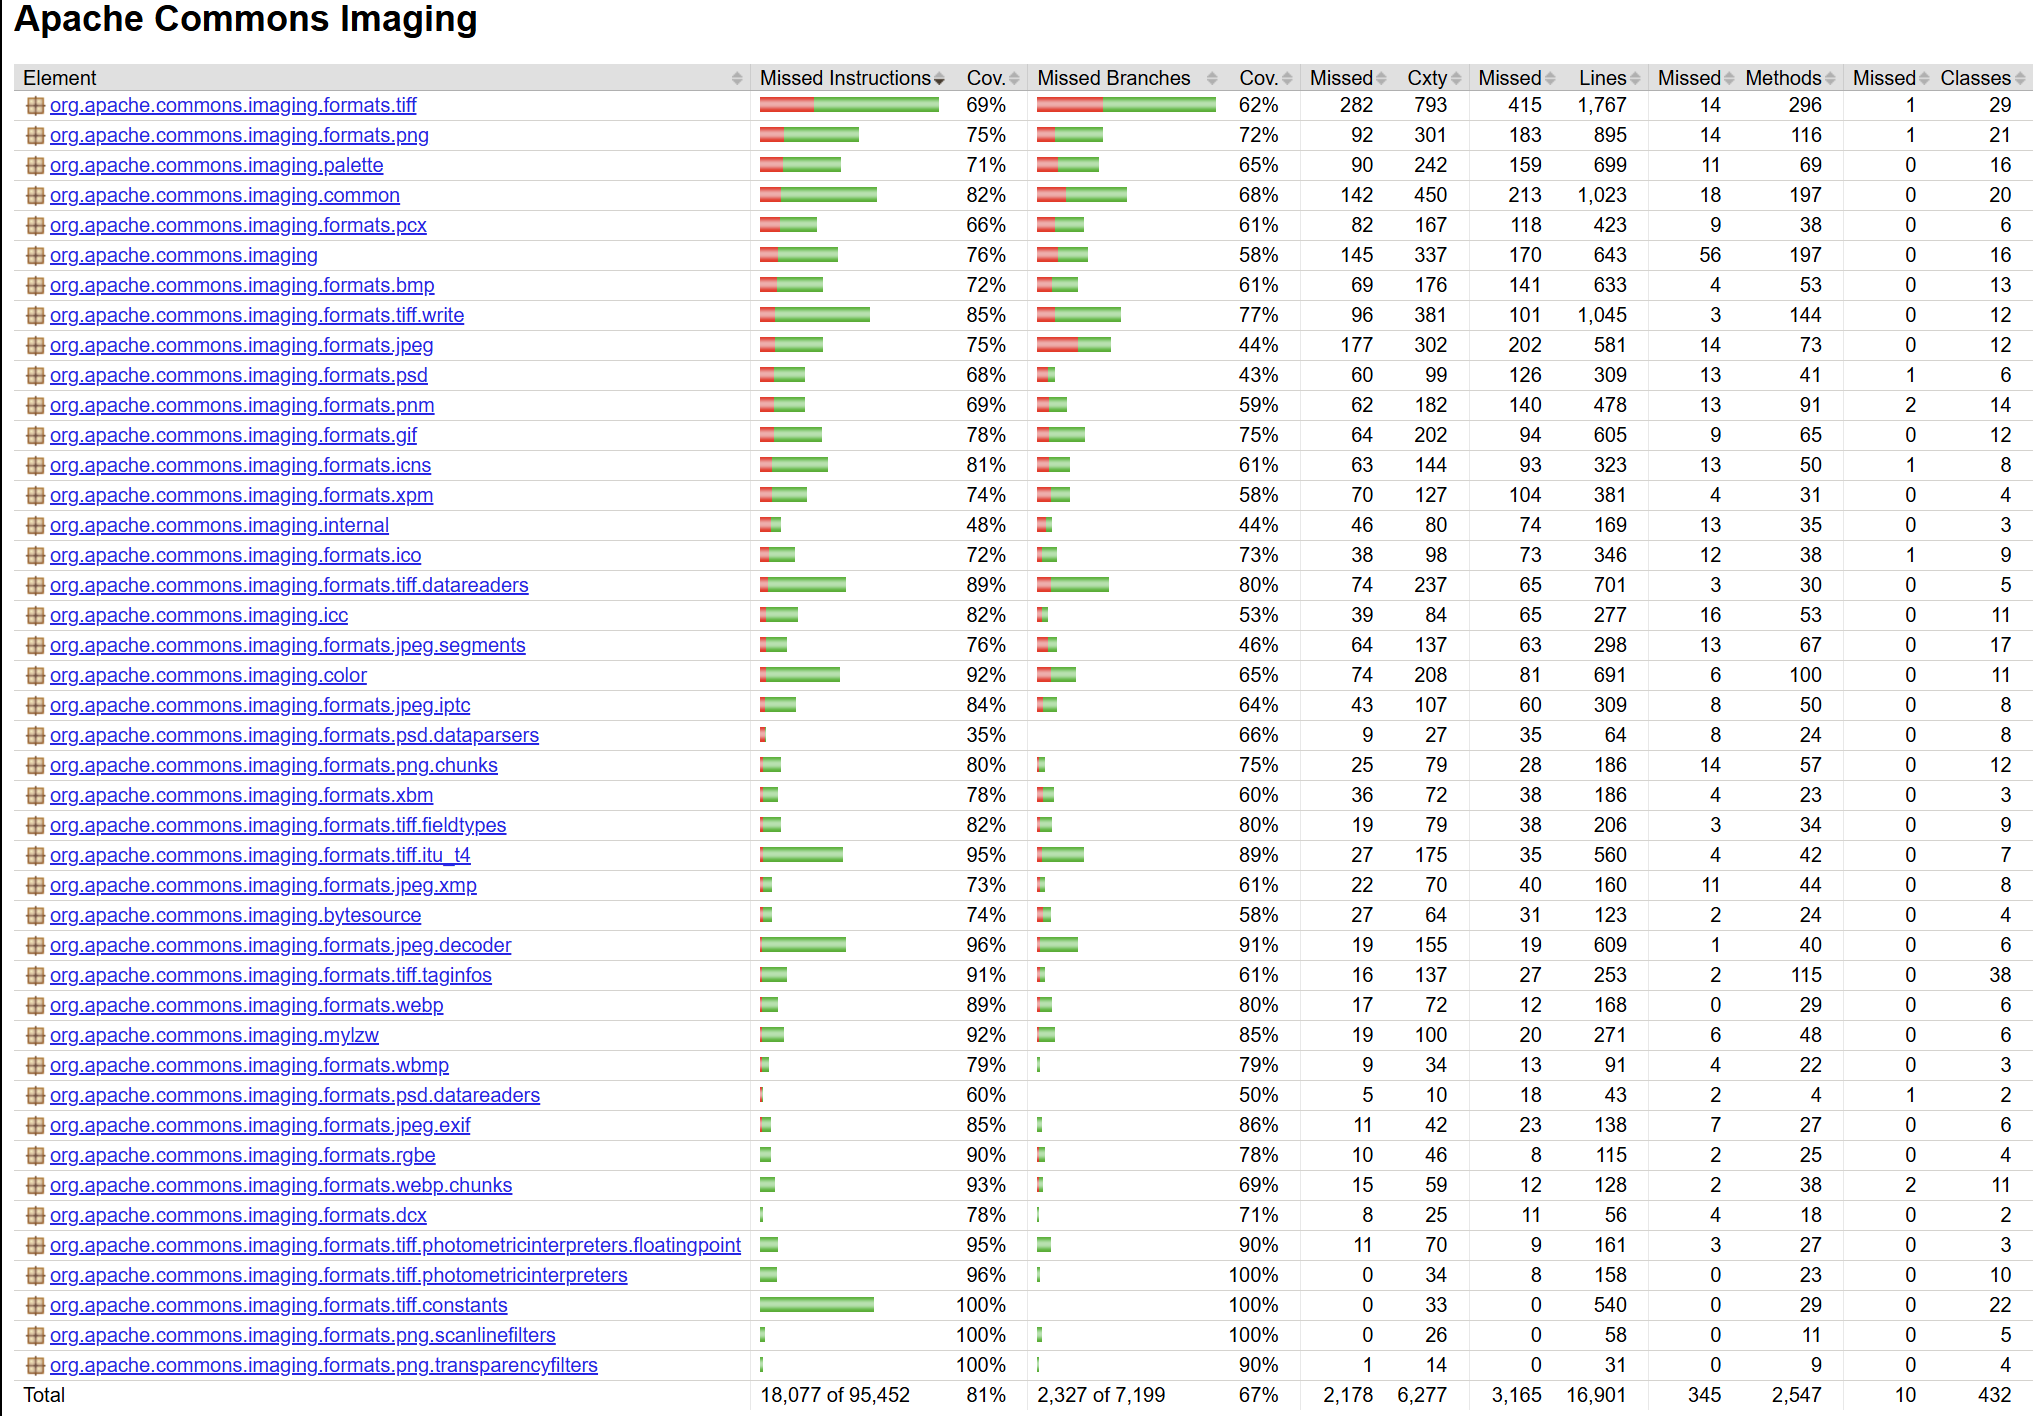
\includegraphics[width=1\textwidth]{Report_Img/final_cov.png}
    \caption{Visualization of Final Code Coverage Results.}
    \label{fig:final_coverage_visualization}
\end{figure}

\noindent The results demonstrate some improvements in test coverage and a reduction in missed methods and classes, indicating better validation of the codebase.

\newpage

% Mutation Testing with PiTest
\chapter{Mutation Testing with PiTest}
Mutation testing is performed to evaluate the effectiveness of the test cases by introducing small modifications (mutations) to the code and ensuring that the tests can detect the changes.

After adding the necessary plugins and dependencies, the following command was run to initiate the mutation testing process:

\begin{lstlisting}[language=bash, caption=Mutation Testing Command]
mvn org.pitest:pitest-maven:mutationCoverage
\end{lstlisting}

\section{Mutation Test Results}
The overall mutation test results for the commons-imaging project are as follows:

\begin{table}[H]
    \centering
    \begin{tabular}{|l|c|c|c|c|c|}
        \hline
        \textbf{Metric} & \textbf{Classes} & \textbf{Line Cov.} & \textbf{Mutation Cov.}& \textbf{Survived Mut.} & \textbf{Test Strength} \\ \hline
        \textbf{Overall} & 69 & 76\% (2973/3904) & 56\% (1993/3564) & 44\% (1571/3564) & 70\% (1993/2839) \\ \hline
    \end{tabular}
    \caption{Mutation Test Results Overview.}
    \label{tab:mutation_results}
\end{table}

The number of survived mutants for the whole project is calculated as:

\begin{quote}
    Survived Mutants = Total Mutants - Killed Mutants \\
    Survived Mutants = 3564 - 1993 = 1571
\end{quote}

\begin{figure}[H]
    \centering
    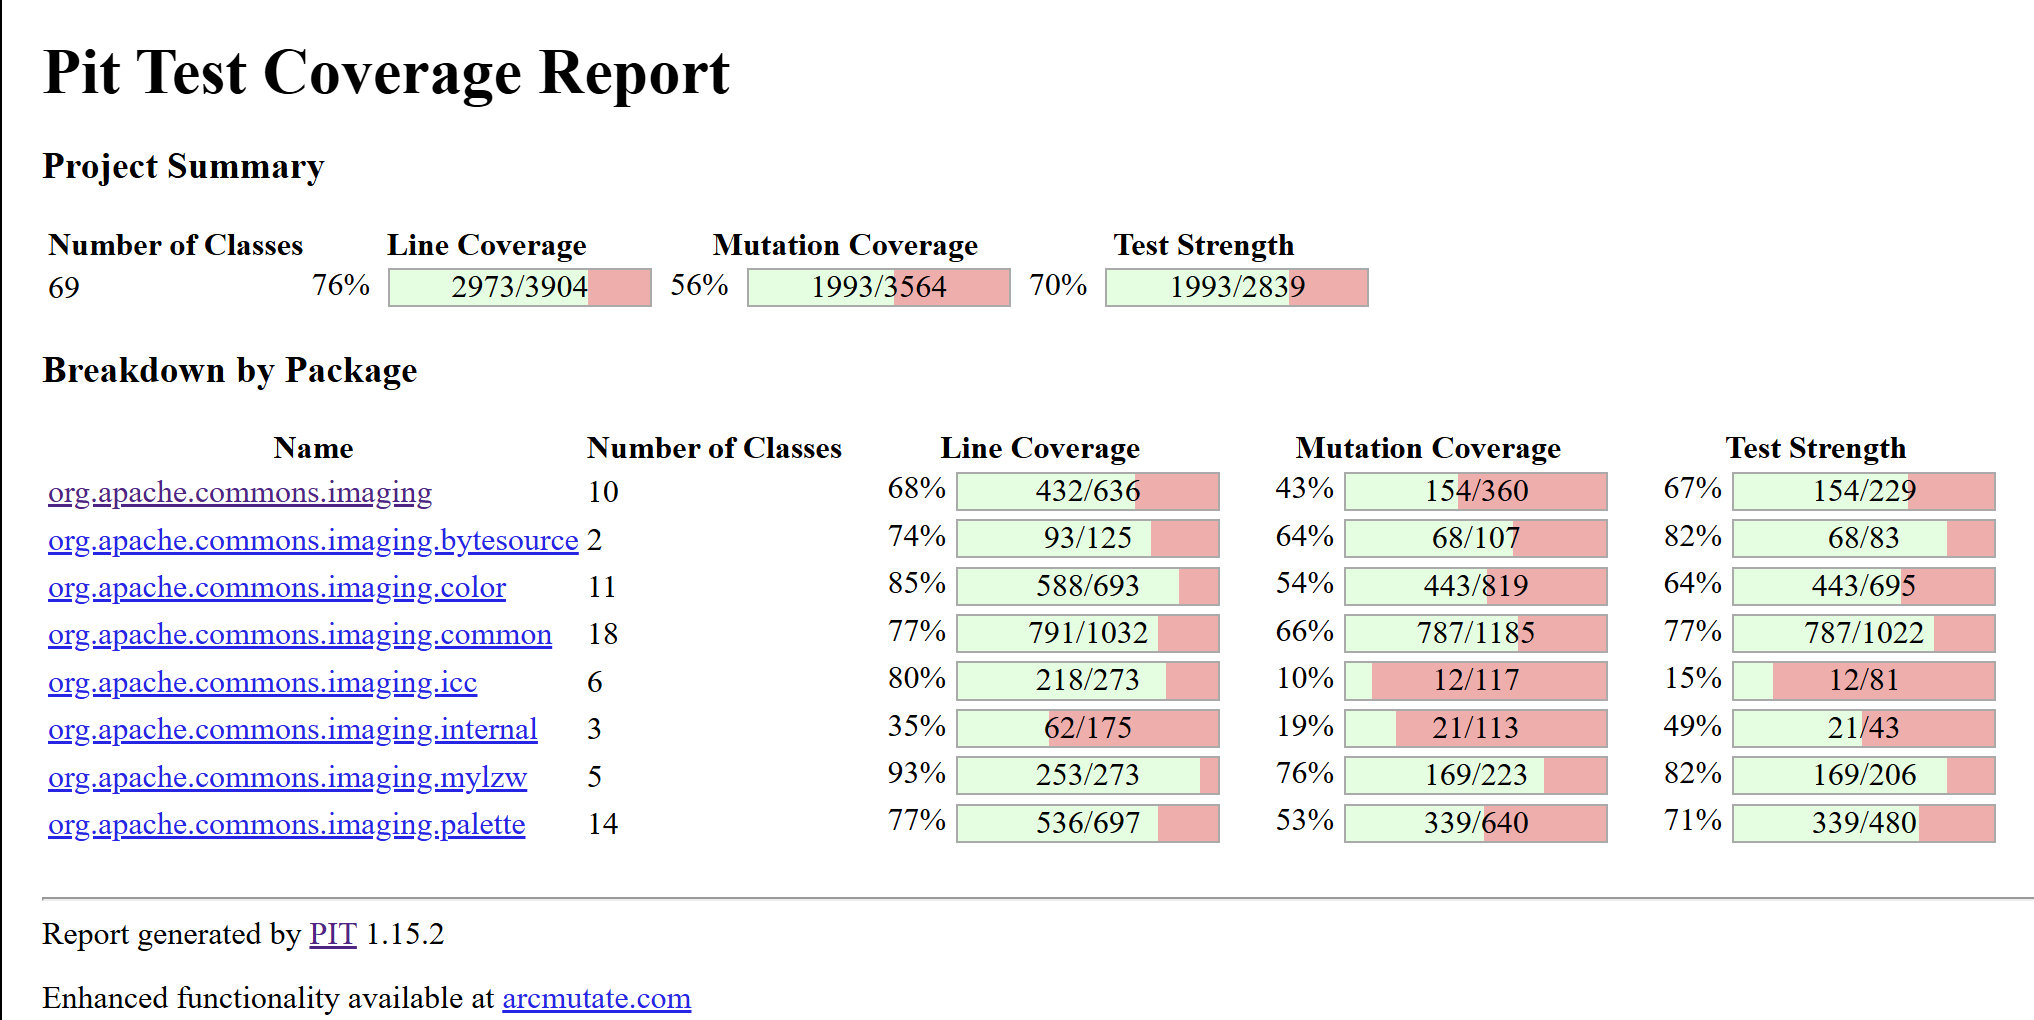
\includegraphics[width=1\textwidth]{Report_Img/pit.png}
    \caption{Visualization of PIT Coverage Results.}
    \label{fig:mutation_coverage}
\end{figure}
\newpage
\section{Detailed Analysis: ColorTools.java}
The results for \texttt{ColorTools.java} before and after adding additional tests (\texttt{ColorToolsTest.java}) were as follows:

\begin{table}[H]
    \centering
    \begin{tabular}{|l|c|c|c|c|c|}
        \hline
        \textbf{Metric} & \textbf{Classes} & \textbf{Line Cov.} & \textbf{Mutation Cov.}& \textbf{Survived Mut.} & \textbf{Test Strength} \\ \hline
        \textbf{Before} & 1 & 0\% (0/62) & 0\% (0/29) & 100\% (29/29)  & Undefined (0/0) \\ \hline
        \textbf{After} & 1 & 60\% (37/62) & 62\% (18/29) & 38\% (11/29)  & 90\% (18/20) \\ \hline
    \end{tabular}
    \caption{Mutation Test Results for \texttt{ColorTools.java}.}
    \label{tab:mutation_results_color_tools}
\end{table}

\noindent The following images show the progress made in terms of test coverage for \texttt{ColorTools.java}:

\begin{figure}[H]
    \centering
    
\includegraphics[width=1\textwidth]{Report_Img/pit_init.png}
    \caption{Initial Coverage and Mutation Results for \texttt{ColorTools.java}.}
    \label{fig:color_tools_initial}
\end{figure}

\begin{figure}[H]
    \centering
    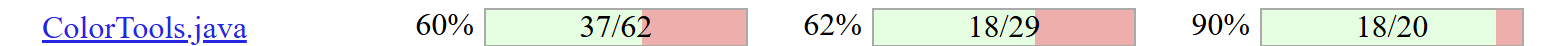
\includegraphics[width=1\textwidth]{Report_Img/pit_final.png}
    \caption{Improved Coverage and Mutation Results for \texttt{ColorTools.java}.}
    \label{fig:color_tools_improved}
\end{figure}

\noindent While 100\% line coverage wasn't achieved, this improvement shows a significant increase in coverage, reducing the number of surviving mutants and improving overall test strength.

\newpage


% Performance Testing with JMH
\chapter{Performance Testing with JMH}
Performance tests are implemented using JMH to identify performance bottlenecks in the commons-imaging project.

\section{Benchmark Setup}
The directory containing the benchmarks is located at:

\begin{lstlisting}[language=bash]
../src/test/java/org/apache/commons/imaging/benchmark
\end{lstlisting}

The following files are part of the benchmark setup:
\begin{itemize}
    \item \texttt{ImagingBenchmark.java}
    \item \texttt{sample.jpg}
    \item \texttt{sample\_baseline.jpg}
    \item \texttt{sample.png}
    \item \texttt{sample.tiff}
    \item \texttt{sample.bmp}
\end{itemize}

The benchmarks were run by first executing the following Maven command:

\begin{lstlisting}[language=bash]
mvn clean install
\end{lstlisting}

Then, the \texttt{ImagingBenchmark} class was run with the following configuration:

\begin{lstlisting}[language=java, caption=ImagingBenchmark-configuration]
@BenchmarkMode(Mode.AverageTime)
@OutputTimeUnit(TimeUnit.MILLISECONDS)
@State(Scope.Thread)
@Fork(1)
@Warmup(iterations = 3)
@Measurement(iterations = 5)
\end{lstlisting}
\newpage
\section{Stress Testing Results}
The most resource-intensive components were stress-tested using JMH, and the results are summarized in the table below:

\begin{table}[H]
    \centering
    \begin{tabular}{|l|c|c|c|}
        \hline
        \textbf{Benchmark} & \textbf{Mode} & \textbf{Score} & \textbf{Units} \\ \hline
        \texttt{ImagingBenchmark.testBmpDecoding} & avgt & 1.157 & ms/op \\ \hline
        \texttt{ImagingBenchmark.testBmpImageInfoRetrieval} & avgt & 0.300 & ms/op \\ \hline
        \texttt{ImagingBenchmark.testBmpImageWriting} & avgt & 8.348 & ms/op \\ \hline
        \texttt{ImagingBenchmark.testImageInfoRetrieval} & avgt & 0.476 & ms/op \\ \hline
        \texttt{ImagingBenchmark.testImageResizing} & avgt & 36.858 & ms/op \\ \hline
        \texttt{ImagingBenchmark.testJpegDecoding} & avgt & 212.311 & ms/op \\ \hline
        \texttt{ImagingBenchmark.testPngEncoding} & avgt & 132.896 & ms/op \\ \hline
        \texttt{ImagingBenchmark.testTiffMetadataExtraction} & avgt & 1.217 & ms/op \\ \hline
    \end{tabular}
    \caption{Stress Testing Results of Commons-Imaging Project.}
    \label{tab:stress_testing_results}
\end{table}


\begin{figure}[H]
    \centering
    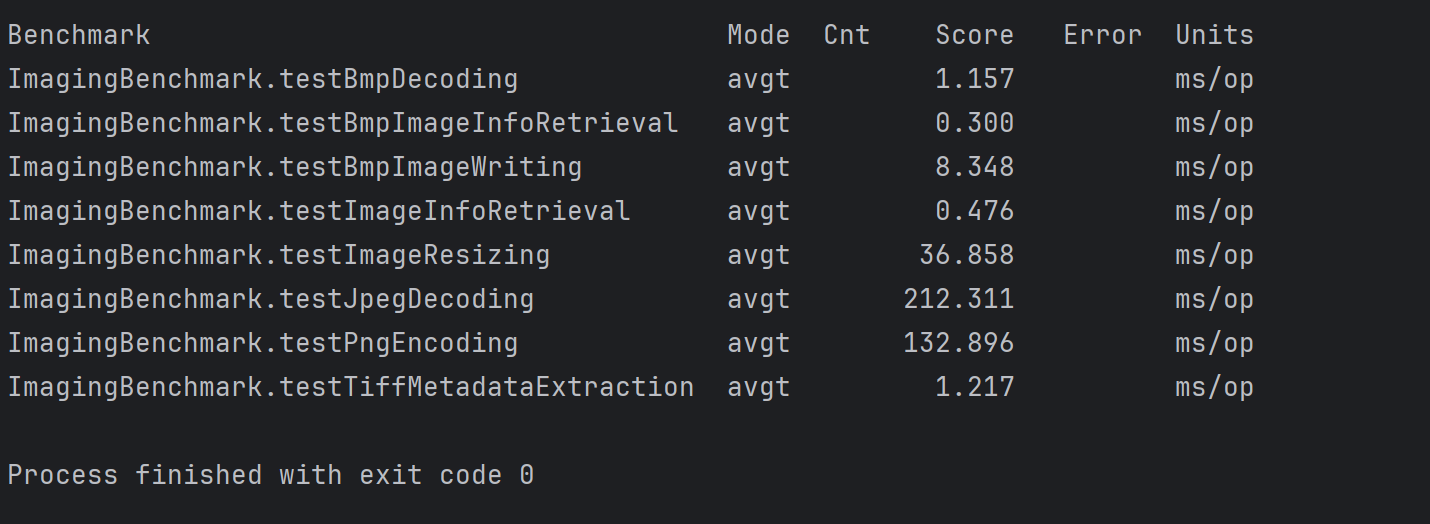
\includegraphics[width=1\textwidth]{Report_Img/benchmark.png}
    \caption{Benchmark Results of Selected Methods of Commons-Imaging Project.}
    \label{fig:benchmark_result}
\end{figure}

\newpage


% Automated Test Generation
\chapter{Automated Test Generation}
Automated tests were generated using Randoop to improve coverage on poorly tested components. These tests focus on edge cases and scenarios not previously covered.

\section{Low Coverage Packages}
From the JaCoCo report, we identified that three packages had low coverage: 
\begin{itemize}
    \item \texttt{internal}
    \item \texttt{formats/psd/dataparsers}
    \item \texttt{formats/tiff}
\end{itemize}
The report also highlights the classes within these packages that need additional test coverage, as shown in the image below:
\begin{figure}[H]
    \centering
    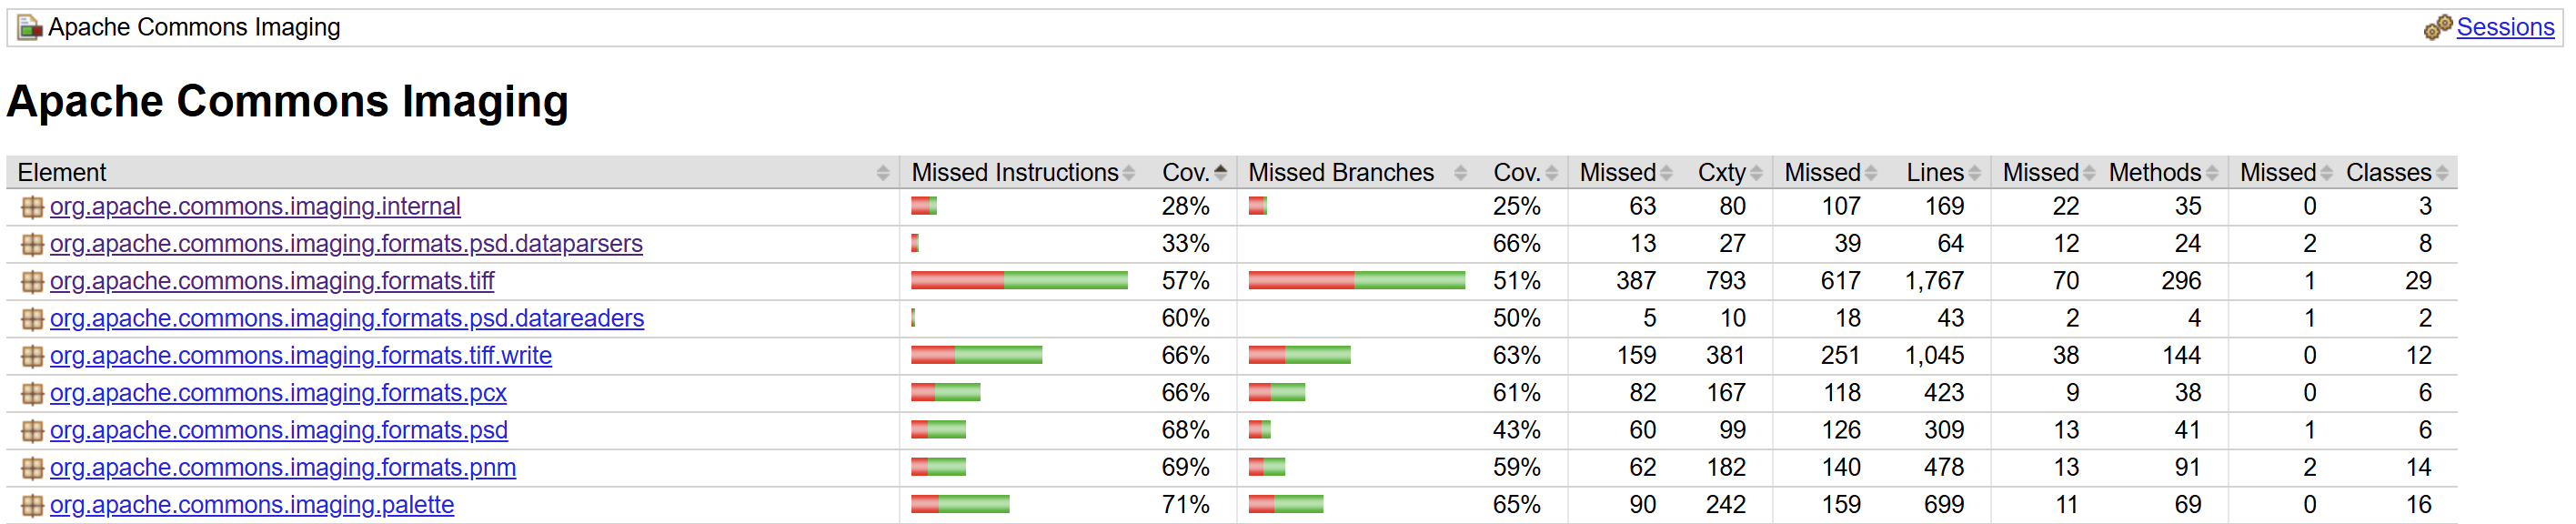
\includegraphics[width=1\textwidth]{Report_Img/auto_gen_init.png}
    \caption{JaCoCo report showing low coverage in specific packages.}
    \label{fig:jacoco-report}
\end{figure}

\section{Test Generation Process}
To generate tests for all the classes within these packages, we first listed the classes using the following commands:

\begin{lstlisting}[language=bash]
cd target/classes
find org/apache/commons/imaging/internal -name "*.class" | sed 's/\//./g' | sed 's/\.class$//'
find org/apache/commons/imaging/formats/psd/dataparsers -name "*.class" | sed 's/\//./g' | sed 's/\.class$//'
find org/apache/commons/imaging/formats/tiff -name "*.class" | sed 's/\//./g' | sed 's/\.class$//'
\end{lstlisting}

These commands search for all `.class` files in the specified directories and convert them into fully qualified class names, which are then copied and saved to a text file called \texttt{Randoop\_Test\_Classes.txt} manually.

\section{Running Randoop}
Once the class names were added to the \texttt{Randoop\_Test\_Classes.txt} file, we ran the following command to generate the tests:

\begin{lstlisting}[language=bash]
java -cp "randoop-all-4.3.2.jar;target/classes" randoop.main.Main gentests $(Get-Content Randoop_Test_Classes.txt | ForEach-Object \{ "--testclass=$\_"\} ) --time-limit=200 --junit-output-dir=src/test/java/org/apache/commons/imaging/randoop/
\end{lstlisting}
\\
This command uses the Randoop tool to generate tests for the classes listed in the text file. The generated tests are stored in the \texttt{randoop} folder and are written in JUnit format.

\section{Test Coverage Improvement}
After generating the tests, we observed an improvement in coverage, as shown in the following image:
\begin{figure}[H]
    \centering
    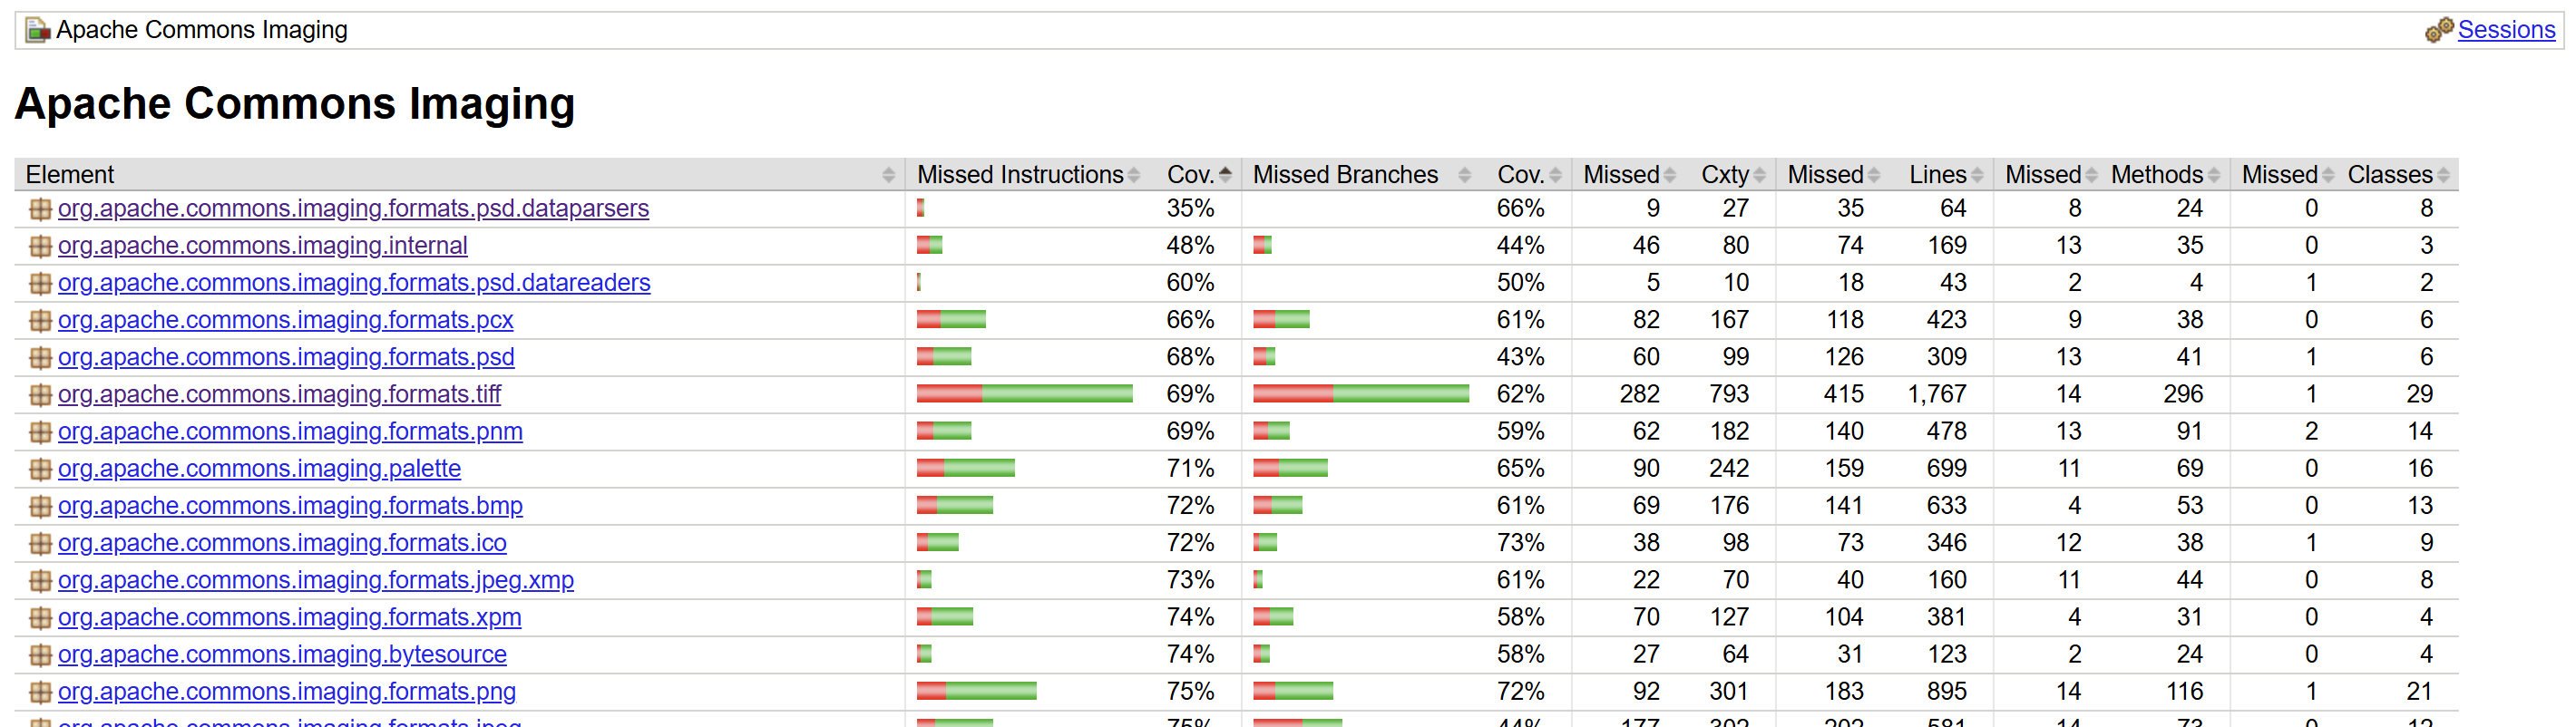
\includegraphics[width=\textwidth]{Report_Img/auto_gen_final.png}
    \caption{Coverage improvement after generating tests using Randoop.}
    \label{fig:coverage-improvement}
\end{figure}

% Table for org.apache.commons.imaging.internal
\begin{table}[H]
    \centering
    \begin{tabular}{|l|c|c|}
        \hline
        \textbf{Metric} & \textbf{Instruction Coverage} & \textbf{Branch Coverage} \\ \hline
        \textbf{Before} & 28\% & 25\% \\ \hline
        \textbf{After}  & 48\% & 44\% \\ \hline
    \end{tabular}
    \caption{Coverage for \texttt{org.apache.commons.imaging.internal}.}
    \label{tab:coverage_internal}
\end{table}

% Table for org.apache.commons.imaging.formats.psd.dataparsers
\begin{table}[H]
    \centering
    \begin{tabular}{|l|c|c|}
        \hline
        \textbf{Metric} & \textbf{Instruction Coverage} & \textbf{Branch Coverage} \\ \hline
        \textbf{Before} & 33\% & 66\% \\ \hline
        \textbf{After}  & 35\% & 66\% \\ \hline
    \end{tabular}
    \caption{Coverage for \texttt{org.apache.commons.imaging.formats.psd.dataparsers}.}
    \label{tab:coverage_psd_dataparsers}
\end{table}

% Table for org.apache.commons.imaging.formats.tiff
\begin{table}[H]
    \centering
    \begin{tabular}{|l|c|c|}
        \hline
        \textbf{Metric} & \textbf{Instruction Coverage} & \textbf{Branch Coverage} \\ \hline
        \textbf{Before} & 57\% & 51\% \\ \hline
        \textbf{After}  & 69\% & 62\% \\ \hline
    \end{tabular}
    \caption{Coverage for \texttt{org.apache.commons.imaging.formats.tiff}.}
    \label{tab:coverage_tiff}
\end{table}

\newpage
\section{Challenges and Limitations}
While this method improved coverage, it has some limitations:
\begin{itemize}
    \item The generated tests often contain redundancy.
    \item It does not guarantee sufficient coverage for all methods.
    \item The process generates more tests than are necessary, leading to inefficiency.
\end{itemize}
Despite these limitations, automated test generation with Randoop provides a valuable first step in improving test coverage, especially for poorly tested components.

\newpage


% Security Analysis with Snyk
\chapter{Security Analysis with Snyk}

\section{Steps to Run Snyk}
To perform security analysis using Snyk, follow these steps:

\begin{lstlisting}[language=bash]
npm install -g snyk
snyk auth
snyk test
snyk test --json > snyk-report.json
\end{lstlisting}

\section{Vulnerability Report}
There were no vulnerabilities found for the commons-imaging project, as seen in the image below. However, there are some vulnerable paths in the web app backend Dockerfile, which will be reported instead.

\begin{figure}[H]
    \centering
    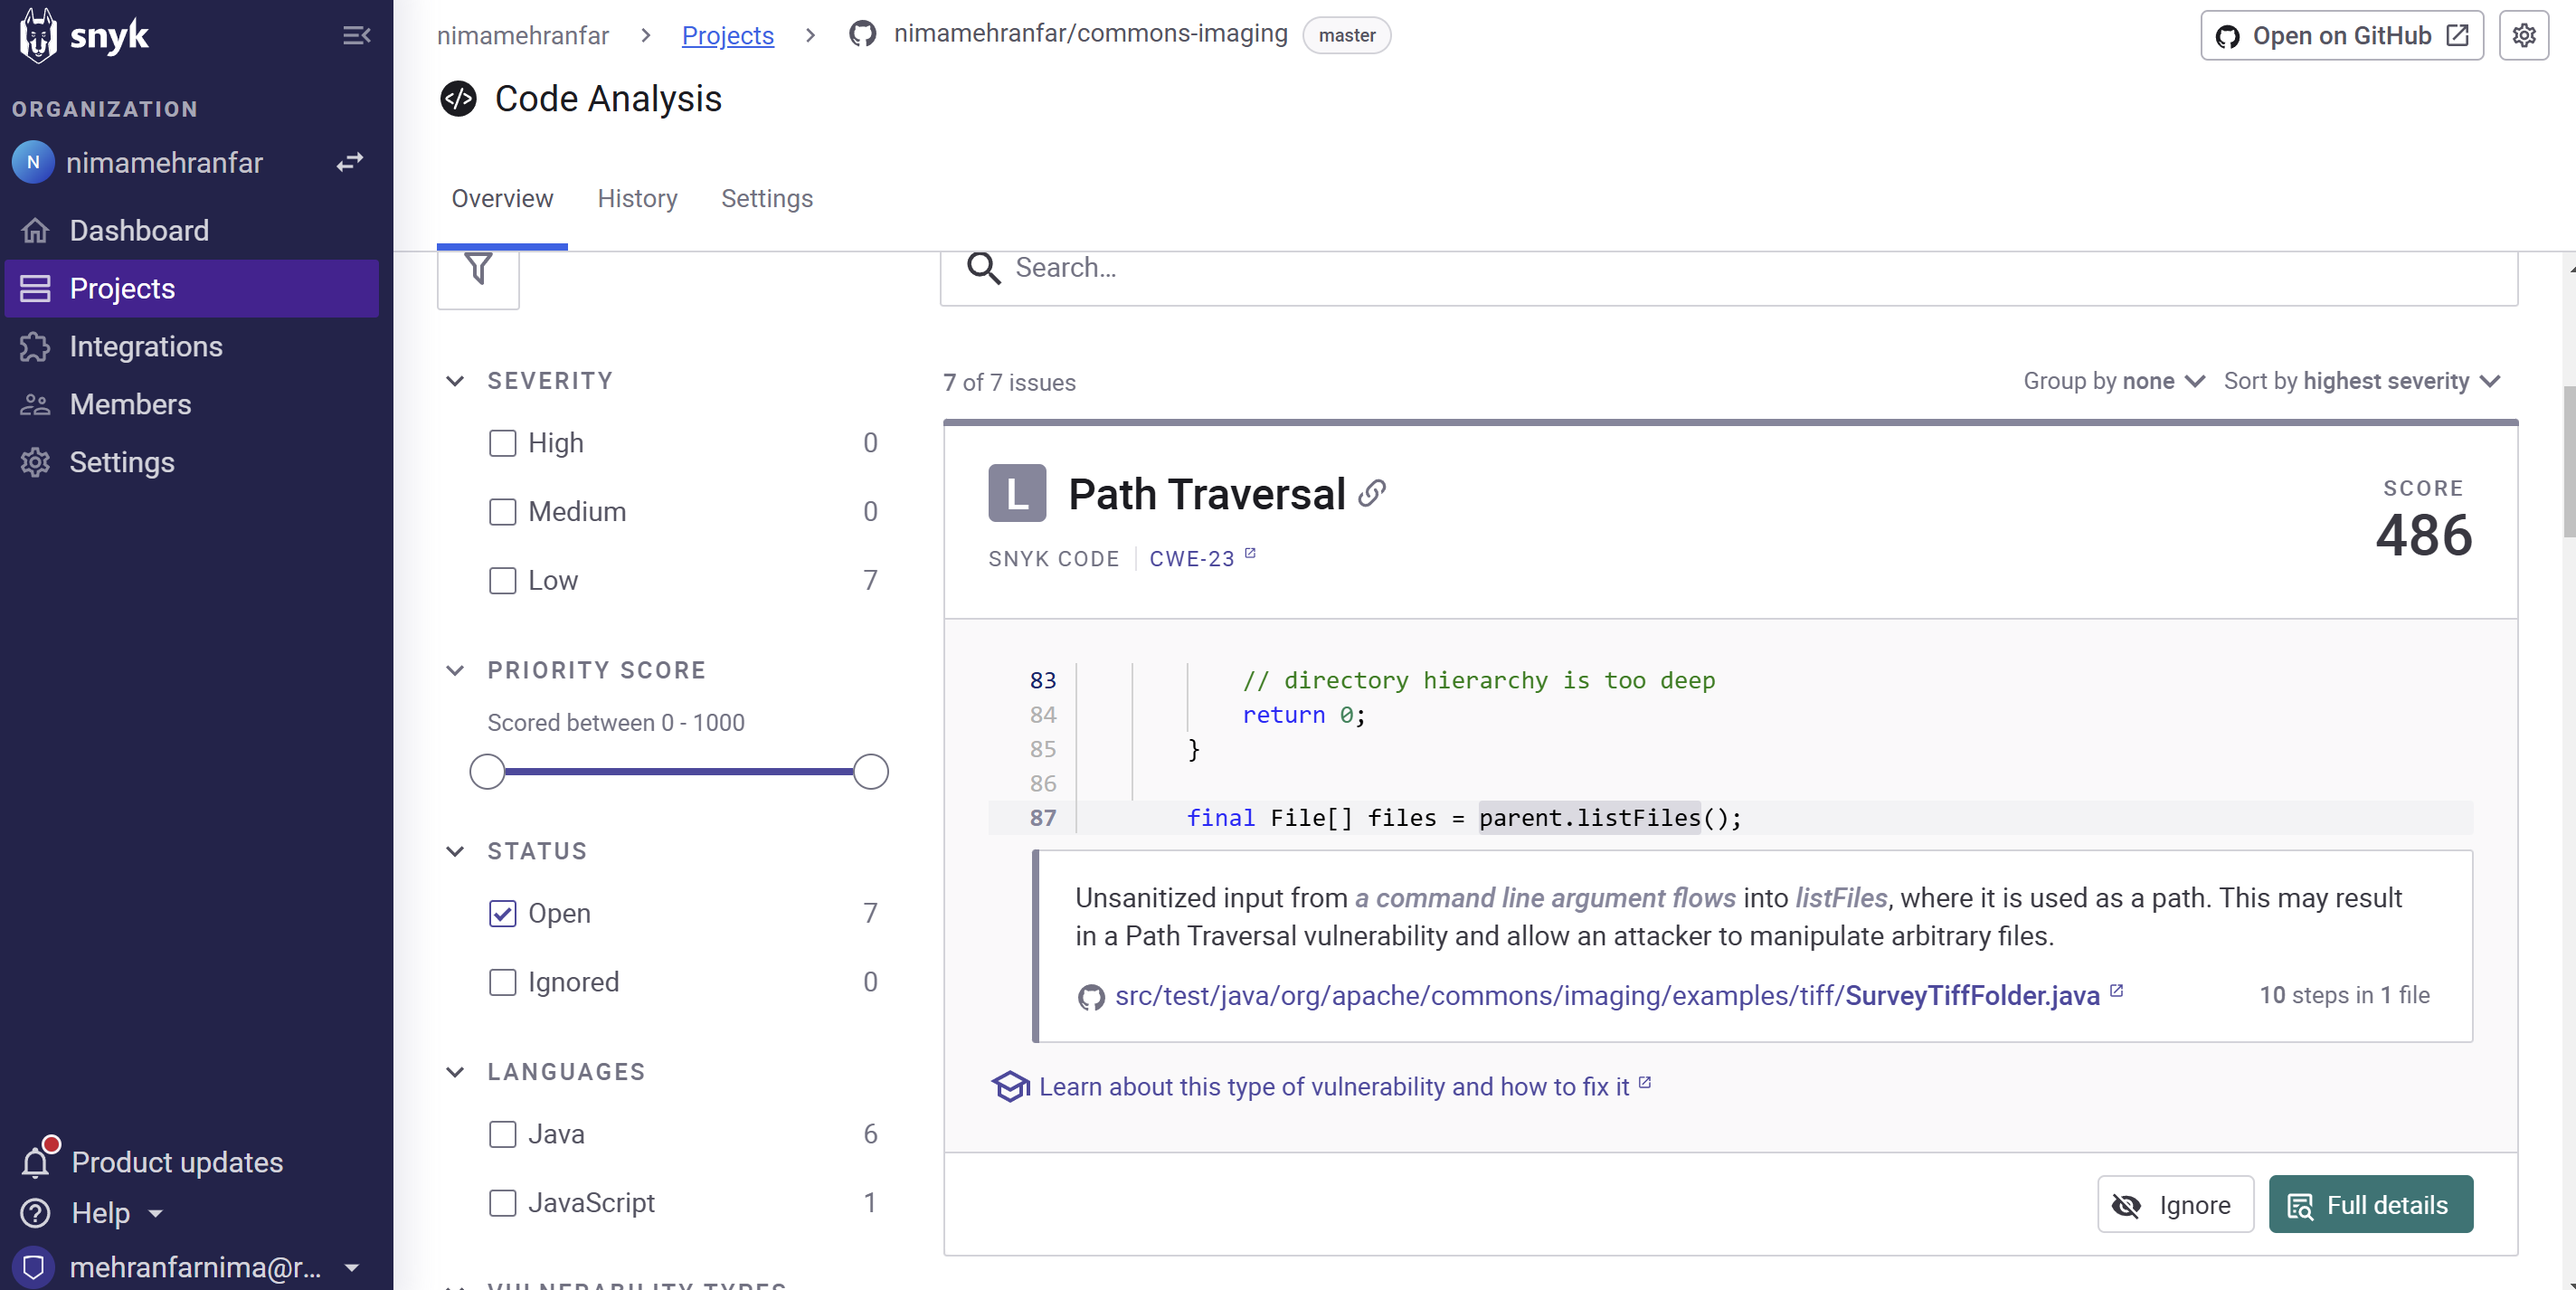
\includegraphics[width=0.65\textwidth]{Report_Img/synk.png}
    \caption{Snyk report showing no vulnerabilities for commons-imaging.}
    \label{fig:snyk-report}
\end{figure}

By changing the OpenJDK version to a newer one, many of the vulnerabilities were resolved, as shown in the image below:

\begin{figure}[H]
    \centering
    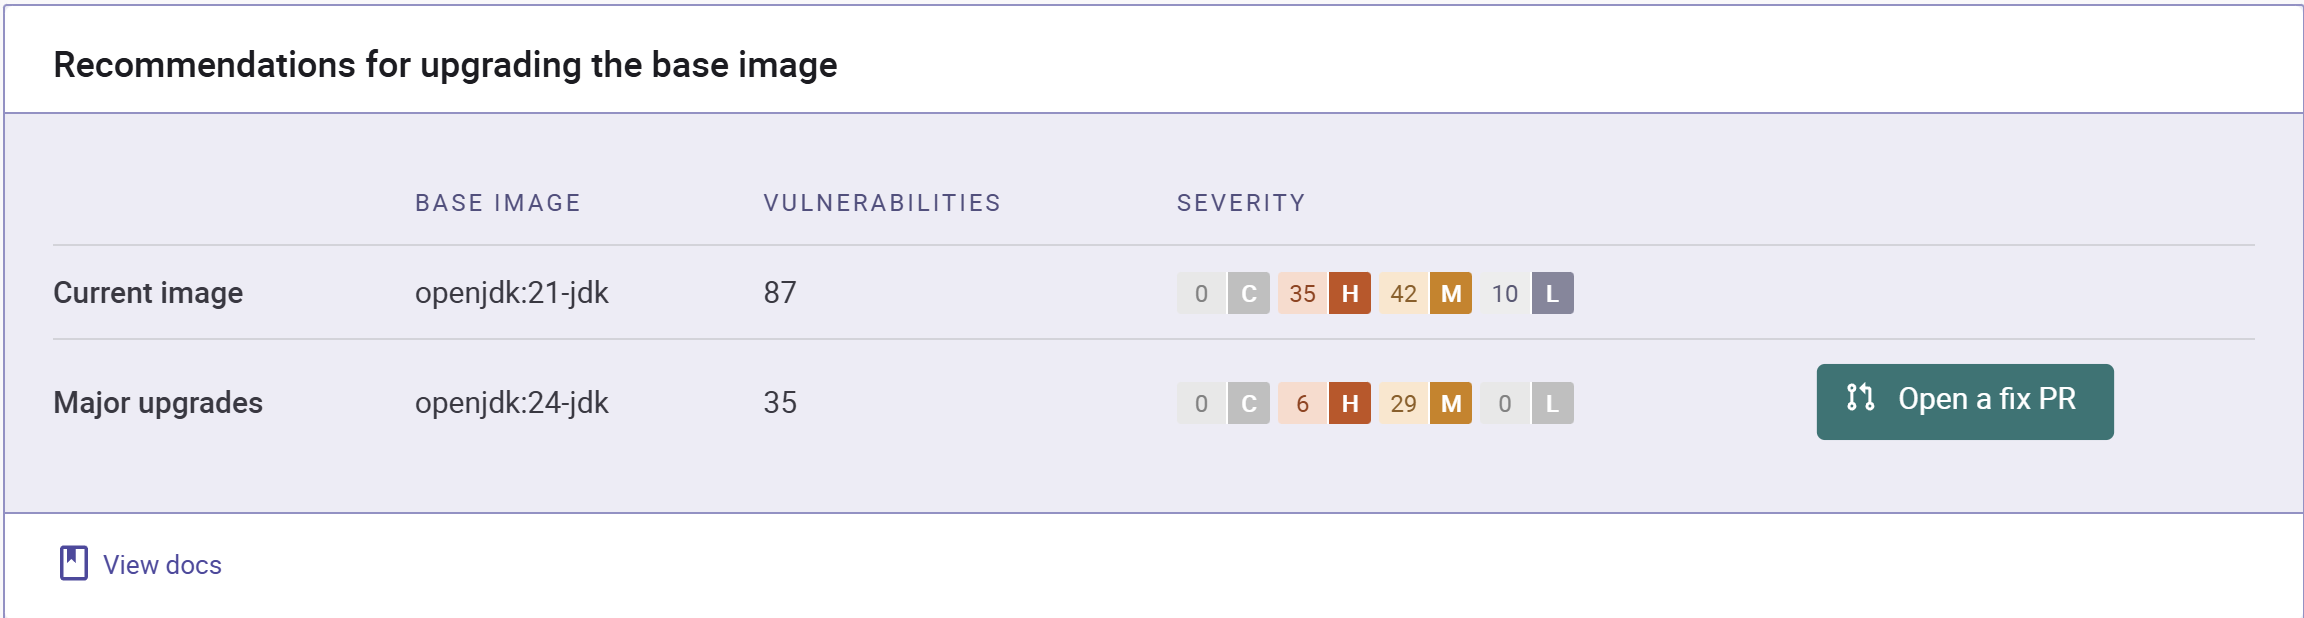
\includegraphics[width=0.65\textwidth]{Report_Img/synk_backend.png}
    \caption{Vulnerabilities reduced after updating the OpenJDK version.}
    \label{fig:openjdk-update}
\end{figure}

\section{Security Issues Found}
During the analysis, the following security issues were identified:
\begin{itemize}
    \item 7 "low" level issues, all of which were related to unsanitized input.
    \item This issues seem to be false positives because the project is an API and utility, and there is no allowed directory. Users can use any directory they want.
    \item However, if we want to limit the user to their current directory, we can fix these issues. For example, unsanitized input from a command-line argument was found in the file \texttt{src/test/java/org/apache/commons/imaging/examples/tiff \\ /SurveyTiffFolder.java:collectPaths.class}, leading to a potential \texttt{Path Traversal} vulnerability.
\end{itemize}

Below is an image showing the identified vulnerability:

\begin{figure}[H]
    \centering
    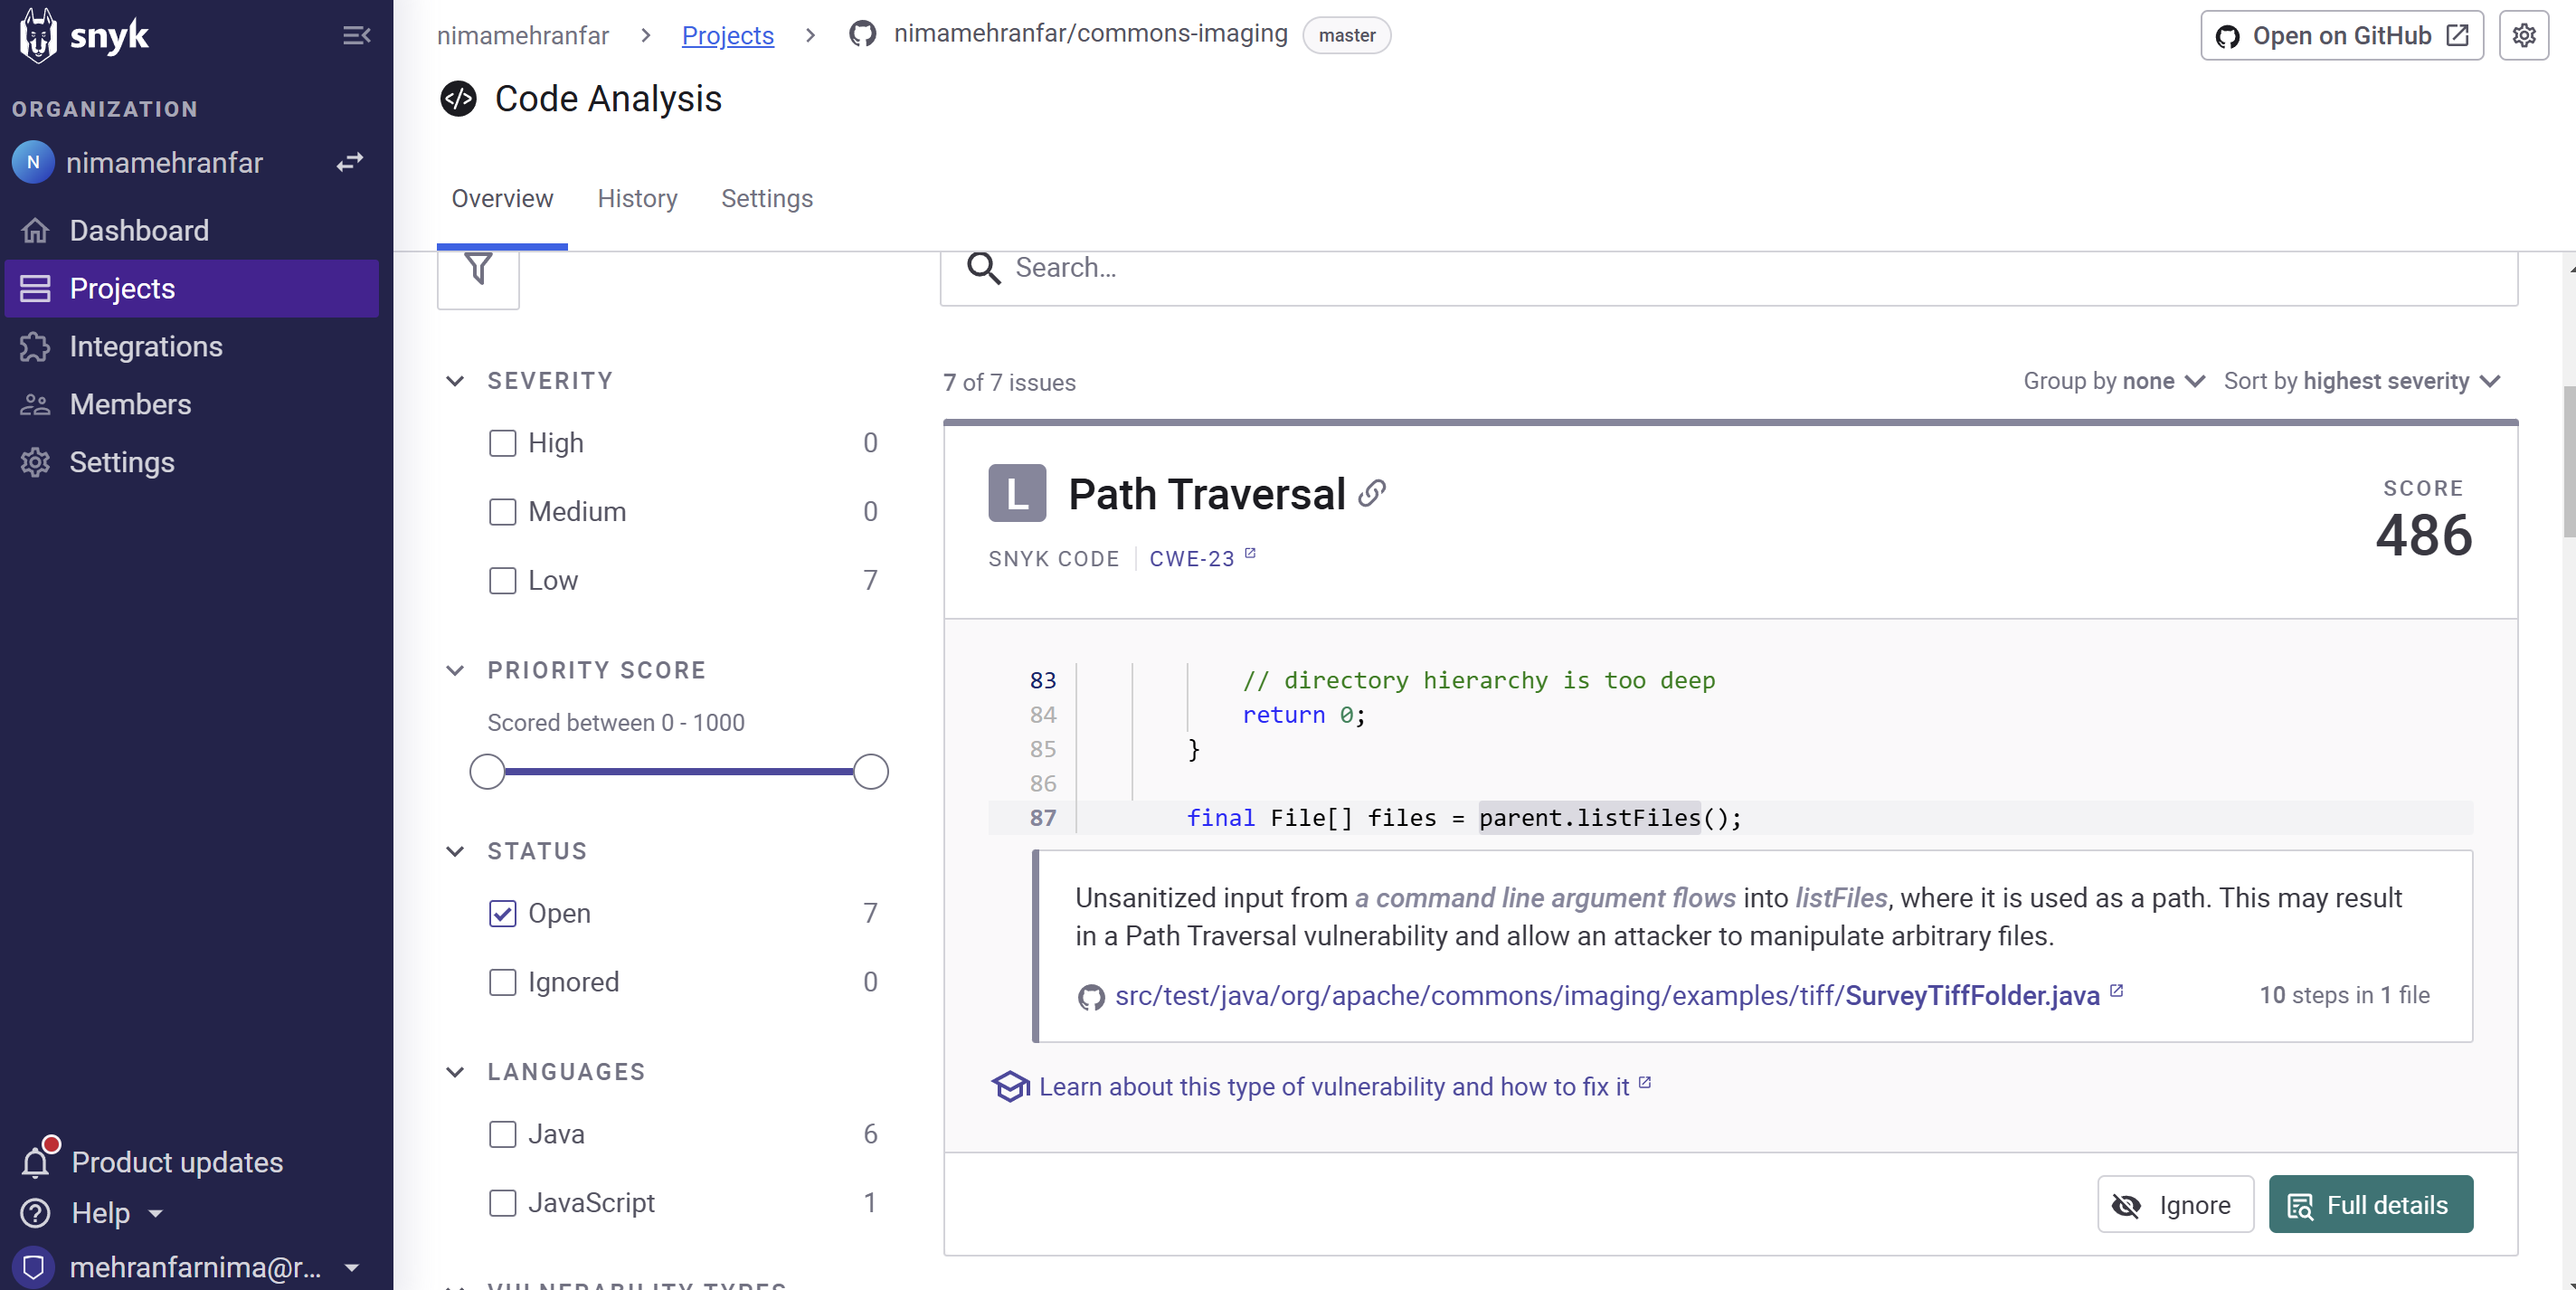
\includegraphics[width=0.65\textwidth]{Report_Img/synk_input_issue.png}
    \caption{Unsanitized input vulnerability found in SurveyTiffFolder.java:collectPaths.}
    \label{fig:unsanitized-input}
\end{figure}

To fix this issue, we can ensure that the file paths remain within the base directory, as shown in the code snippet below:

\begin{lstlisting}[language=java, caption=SurveyTiffFolder.java:collectPath.class fix]
private static final String BASE_DIRECTORY = System.getProperty("user.dir");

private static boolean isWithinBaseDirectory(File file) throws IOException {
    // Get the canonical path of the file
    String canonicalPath = file.getCanonicalPath();
    String baseDirectoryPath = new File(BASE_DIRECTORY).getCanonicalPath();

    // Check if the canonical path starts with the base directory path
    return canonicalPath.startsWith(baseDirectoryPath);
}

private static int collectPaths() {
    ...
    try {
        // Resolve the file's canonical path to get the absolute path
        File canonicalFile = f.getCanonicalFile();

        // Normalize the path and ensure it is within the base directory
        if (!isWithinBaseDirectory(canonicalFile)) {
            continue; // Skip files outside the base directory
        }

        final String[] temp = Arrays.copyOf(scratch, depth + 1);
        pathList.add(temp);
    } catch (IOException e) {
        // Handle any IOExceptions (e.g., if getCanonicalPath fails)
    }
    ...
}
\end{lstlisting}

This fix ensures that the file operations are limited to the base directory, preventing path traversal vulnerabilities. 
\\
All other identified issues can be fixed in a similar manner if they are not false positives, by sanitizing the inputs and ensuring that file operations are safe.

\newpage


% Conclusion
\chapter{Conclusion}
The commons-imaging project underwent various quality assurance practices. Through CI/CD pipeline integration, refactoring based on SonarCloud issues, performance and mutation testing, and security analysis, we have significantly improved the project’s code quality and created a test Docker for it. Future work will depend on project developers focusing on addressing any remaining vulnerabilities and expanding the test coverage.
\\ \\
The source code for this project is available at \href{https://github.com/nimamehranfar/commons-imaging}{\texttt{GitHub Repository}}.

\newpage

% References
\chapter{References}
\begin{itemize}
    \item SonarCloud Documentation: \url{https://sonarcloud.io/}.
    \item Docker Documentation: \url{https://docs.docker.com/}.
    \item JaCoCo Documentation: \url{https://www.jacoco.org/jacoco/}.
    \item PiTest Documentation: \url{https://pitest.org/}.
    \item JMH Documentation: \url{https://openjdk.java.net/projects/code-tools/jmh/}.
    \item Randoop Documentation: \url{http://randoop.github.io/}.
    \item Snyk Documentation: \url{https://snyk.io/}.
    \item ChatGPT: \url{https://chatgpt.com/}.
\end{itemize}

\end{document}
